%%%%%%%%%%%%%%%%%%%%%%%%%%%%%%%%%%%%%%%%%%%%%%%%%%%%%%%%%%%%%%%%%%%%%
%%% Hochschule Hamm-Lippstadt
%%%
%%% Erstellt:      Luis Koch und Fabian Babik
%%%%%%%%%%%%%%%%%%%%%%%%%%%%%%%%%%%%%%%%%%%%%%%%%%%%%%%%%%%%%%%%%%%%%

%%%%%%%%%%%%%%%%%%%%%%%%%%%%%%%%%%%%%%%%%%%%%%%%%%%%%%%%%%%%%%%%%%%%%
%%% 
%%% Einstellungen
%%%
%%% Benoetigt wird KOMA-Skript ab Version 2.8j vom 30.07.2001
%%% Vor der Veraenderung irgendwelcher Einstellungen wird dringend empfohlen
%%% die Anleitung zum KOMA-Skript (scrguide) zu konsultieren !!
%%%
%%% Bilder bitte nicht mit Endung einbinden, so ist die Erzeugung von
%%% DVI, PS und PDF problemlos möglich!
%%% Infos zur \documentclass:
%%% http://wannert.net/latex/eine-praeambel-nicht-nur-fuer-mathematiker
%%%
%%%%%%%%%%%%%%%%%%%%%%%%%%%%%%%%%%%%%%%%%%%%%%%%%%%%%%%%%%%%%%%%%%%%%

% Haupteinstellungen für die KOMA-Dokumentenvorlage
% ===================================================
\documentclass[    
            paper=a4, 		%Papiergröße
            %----------------------------------------------
            %DIVcalc,        % Automatische Berechnung des Satzspiegels nach "goldenem Schnitt"
            DIV15,         % Unterteilung des Seitenlayouts in xy Streifen,
                           % führt zu kleineren Rändern, je größer die Zahl.
            %----------------------------------------------
            oneside,        % Seitenaufteilung: einteilig.
            %twoside,         % Seitenaufteilung: zweiseitig.
            %----------------------------------------------
            titlepage,      % Titelseite speziell, ohne Seitenkopf und -fu{\ss}
            %----------------------------------------------
            fontsize=12pt,           % Schriftgröße
            %----------------------------------------------
            %openright,      % Kapitel beginnen nur auf rechten Seiten.
            openany, 				% Kapitel können auf geraden und ungeraden Seiten beginnen
            %----------------------------------------------
            headinclude,    % Kopfzeile wird Seiten-Layouts mit beruecksichtigt
            %----------------------------------------------
            headsepline,    % Linie unter Kolumnentiteln an
            %headnosepline,  % Linie unter Kolumnentiteln aus
            %----------------------------------------------
            %footexclude,    % Fu{\ss}noten-Bereich ausschalten?
            footinclude=false,
            %----------------------------------------------
            footsepline = false,    % Linie über Fußzeilen
            %----------------------------------------------
            headings = normal, % überschriftengröße (Kapitel,...), "big"
            %----------------------------------------------
            fleqn,          % Gleichungen linksbündig statt mittig
            %----------------------------------------------
            %chapterprefix,  % Prefix für Kapitel: "Kapitel"
            %nochapterprefix,% Prefix für Kapitel: keiner.
            %----------------------------------------------
            %halfparskip*,    % Zeilenabstand zwischen Absätzen: mind. 0.25 Zeile
            %halfparskip,    %  Zeilenabstand zwischen Absätzen: 0.5 Zeile
            %parskip,        % Zeilenabstand zwischen Absätzen: 1 Zeile
            %parindent,      % Zeilenabstand zwischen Absätzen: keiner, nur Wort einrücken.
            parskip=half,
            %----------------------------------------------
            german,         % Sprache
            %----------------------------------------------
            %final,          % Version: Endversion
            %draft,          % Version: Zwischenversion, z.~B. ohne Bilder,...
            draft=false,
            %----------------------------------------------
            bibliography = totoc,       % Literaturverzeichnis ins Inhaltsverzeichnis
            %----------------------------------------------
            %pdftex,         % Verwendung mit pdftex
            %----------------------------------------------
            %'BCOR12mm,version=first,       % ergibt links einen Rand von  zusätzlich 1cm zum Binden.
            %----------------------------------------------
            numbers = noenddot,    % Kapitelnummern immer ohne Punkt
            %----------------------------------------------
            caption = tableh,   % korrekte Abstaende bei TabellenUEBERschriften
            %----------------------------------------------
            %abstracton,    % Zusammenfassung?
            %----------------------------------------------
            %draft               % Keine Bilder in der Anzeige, overfull hboxes werden angezeigt
            %----------------------------------------------
                ]{scrbook}[2001/07/30]   % scrbook-Version mind. 2.8j von 2001/07/30
                %]{scrreprt}


% Schalter definieren 
%---------------------------------------------------------
\usepackage{ifthen}
\newboolean{VersionDozent}
\setboolean{VersionDozent}{false}

\newboolean{alphaDIN}
\setboolean{alphaDIN}{true}

% Seitenlayout ändern
% ====================
%\typearea{18}
%\typearea[18mm]{19}          % [Binderand]{Divisor für Seitenaufteilung}
%\areaset[1cm]%               % Zusaetzlicher Rand fuer die Bindung
%        {18cm}{25cm}         % Textbreite und Hoehe


\usepackage{lscape}           % Seite im Querformat bei Erhalt der Kopfzeile
%\usepackage{portland}
\usepackage{rotating} 				% um Text u.s.w. zu rotieren


% Grafiken:
% ==========
\usepackage{ae}                  % Für PDF-Erstellung
\usepackage{graphicx}            % zum Einbinden von Grafiken
\usepackage{float}               % u.a. genaue Plazierung von Gleitobjekten mit H
\graphicspath{{bilder/}{Bilder/}} 			 	 % Verzeichnis, in dem die ganzen Bilder liegen
\usepackage{flafter} 						 % Gleitobjekte immer hinter ihrem ersten Verweis platzieren
%\usepackage{wrapfig} % Bilder mit Text drumrum, Einbinden mit \begin{wrapfigure}
% \usepackage{pstricks}          % PostScript Macros

% pdf-Bilder mit Verwendung von pdf-Latex
%\usepackage[pdftex]{graphicx}
%\usepackage[pdftex,hypertexnames=false]{hyperref}

% Farben vordefinieren
\usepackage{color}
    \definecolor{darkred}{rgb}{0.5,0,0}
    \definecolor{darkgreen}{rgb}{0,0.5,0}
    \definecolor{darkblue}{rgb}{0,0,0.5}
    \definecolor{Hellgrau}{gray}{0.92} 


% Tabellen
% =========
\usepackage{multirow} % Tabellen-Zellen über mehrere Zeilen
\usepackage{ragged2e} %Ausrichtung rechtsbündig möglich mit Option >{\RaggedRight}p{6cm}
\usepackage{longtable} %für 2-Seitige Tabellen

% Für Farben in Tabellen:
\usepackage{colortbl} 



% Bildunterschriften
% ===================
\usepackage{caption, here} % offenbar für neue MikTex-Vers. (z. B. 2.7)


\renewcommand{\captionfont}{\small\itshape} % Bildunterschriften kleiner und kursiv

% Für mehrere Abbildungen in einer:
\usepackage{subfig} %offenbar für neue MikTex-Vers. (z. B. 2.7), funktioniert aber nicht mit den captions (warum???)


% Bei Miktex 2.7 werden die Captions von Subfigures zu breit!
% daher oben subfig laden und hiermit einstellen:
\captionsetup[subfloat]{%
   margin = 4mm,
   labelfont = {it},
   format = plain, % oder 'hang'
   indention = 0em,  % Einruecken der Beschriftung
   singlelinecheck = true, % false (true=bei einer Zeile immer zentrieren)
 }
%}

\captionsetup{
   margin = 4mm,
   %font = {small,rm},
   labelfont = {it},
   format = plain, % oder 'hang'
   indention = 0em,  % Einruecken der Beschriftung
}


% Rechtschreibung 
% ================
\usepackage{ngerman} % neue Rechtschreibung
\usepackage[utf8]{inputenc}    % Input-Encodung: utf-8 fuer Windows
\usepackage{verbatim}          % Quellcode einbinden (\verbatiminput)
\usepackage[T1]{fontenc}         % T1-kodierte Schriften, korrekte Trennmuster fuer Worte mit Umlauten XXX ACHTUNG XXX bringt aber auch mit sich, dass die Auflösung im pdf nicht unendlich ist!!


% Besondere Zeichen
% ==================
% Matrizenbefehle benutzen, für alle Symbole (Mathe)
\usepackage[centertags]{amsmath} % AMS-Mathematik, centertags zentriert Nummer bei split
\usepackage{amsfonts}
\usepackage{amssymb}
\usepackage{amsbsy}

% verschiedene Symbole
%\usepackage{latexsym}           % verschiedene Symbole
\usepackage{textcomp}           % verschiedene Symbole

%für Laplace-Transformationen
\usepackage{trsym, trfsigns}

% für Einheiten
\usepackage{units}

% eingekreiste Zahlen \ding{172} = 1
%\usepackage{psnfss} %wurde nicht gefunden
\usepackage{pifont}

% Häkchen (\checked), Smileys (\smiley),...
%\usepackage{wasysym}

% Kreuz \XSolid, \XSolidBrush
%\usepackage{bbding}

% für z.~B. "N" als Symbol für natürliche Zahlen.
\usepackage{dsfont} %\mathds{N} --> N dann im pdf nicht sichtbar?


% Verzeichnisse, Referenzen
% ==========================
\usepackage{nomencl} 					 % Erstellung einer Nomenklatur
%\usepackage{cite}              % Sortierte und zusammengefasste Zitatnummern 
\usepackage{varioref}          % Verbesserte Referenzen
% \usepackage[numbers, sort]{natbib} % DIN Literaturverzeichnis; nicht zusammen mit cite verwenden!

% Inhaltsverzeichnis: Anzeigetiefe
\setcounter{tocdepth}{3}						%Tiefe des Inhaltsverzeichnisses

% Kopf- und Fußzeilenlayout
% ==========================
\usepackage[left=2cm, right=1.5cm, top=1.5cm, bottom=2cm]{geometry}

\usepackage[automark]{scrlayer-scrpage}
%[] für die erste Seite,{} für alle anderen
\pagestyle{scrheadings}
\clearscrheadfoot                   % Standarddefinitionen l\"{o}schen
\ihead[]{\headmark}                 % Kolumnentitel oben innen
\ohead[\pagemark]{\pagemark}        % Seitennummern immer oben aussen


% BibTex nach DIN1505
\usepackage{bibgerm}    %BibTex German Style DIN 1505

% Seitenlayout
% =============

% damit die erste Zeile eines Absatzes nicht mehr eingerückn wird:
%\parindent0cm

% Werte ändern
\setlength{\parskip}{0.15cm} % Abstand von Absatz zu Absatz (mit leerer Zeile induziert)
\setcounter{secnumdepth}{3} %damit auch Subsubsections nummeriert werden (Nummerierungstiefe)

% Zeilenabstand einstellen:
\usepackage{setspace}            % Zeilenabstand einstellbar
\onehalfspacing                  % eineinhalbzeilig einstellen
%\renewcommand{\baselinestretch}{1.1}

% Das soll weniger Warnungen over/underfull hbox mit sich bringen.
%\sloppy
%\fuzzy  % schaltet \sloppy wieder aus.

% Vordefinierte Namen ändern (Kapitel, ...)
\renewcommand{\bibname}{Literatur} % Literaturverzeichnis wird zu Literatur
\renewcommand{\figurename}{Bild}   % Abbildung wird zu Bild
\renewcommand{\listfigurename}{Bildverzeichnis}


% Schriftart ändern
% ==================
% Serifenlose Schrift als Standard (auch fuer Bildunterschriften!)
\renewcommand{\rmdefault}{cmss}

% Schrift mit Serifen auch fuer Ueberschriften benutzen
%\renewcommand*{\sectfont}{\bfseries}
%\renewcommand*{\descfont}{\bfseries}

\renewcommand{\headfont}{\normalfont\sffamily}    % Kolumnentitel serifenlos
\renewcommand{\pnumfont}{\normalfont\sffamily}    % Seitennummern serifenlos


% Hyperreferenzen -> Links im dvi- und pdf-Dokument
% ==================================================
\usepackage{ifpdf} %ermöglicht das Umschalten von pdf nach eps,...

% Je nach Kompilierung (mit pdf oder mit eps) hier
% automatische Umschaltung.
\ifpdf
    \usepackage[pagebackref,pdftex]{hyperref}
    \pdfcompresslevel=0
\else
    %für Hyperreferenzen im pdf-Dokument, alte Miktex-Version (2.1)
    \usepackage[pagebackref,hypertex]{hyperref}
    % neue Miktex-Version(2.5)
    %\usepackage[a4paper,pagebackref,final,hypertex]{hyperref} %so gehen die Hyperreferenzen in YAP wieder.
\fi

% Hyperreferenzen gezielt einstellen: Farben, Darstellung des pdfs,...
\hypersetup{
    pdftitle        = {Titel},
    pdfsubject      = {Skript},
    pdfauthor       = {Autor},
    pdfkeywords     = {},
    pdfcreator      = {pdftex},
    pdfproducer     = {LaTeX am \today},    linkcolor       = darkred,
    anchorcolor     = darkred,
    citecolor       = darkred,
    filecolor       = darkred,
    menucolor       = darkred,
    urlcolor        = darkred,
%    pdfview         = FitV,
%    pdfstartview    = FitV,
%    pdfstartpage    = {1},
%    pdfpagelayout   =TwoColumnRight,
    pdfpagemode     = UseNone,
    breaklinks      = true,
    colorlinks      = true,
    pdfborder       = 0 0 0,
    plainpages      = false,
%    pdfborder       = 0 0 0,
%    bookmarksnumbered = true,
%    bordercolor     = false,
%    linkbordercolor = {0 0 0},  %Farbe der Textbox
%    citebordercolor = {0 0 0},
%    filebordercolor = {0 0 0},
%    pagebordercolor = {0 0 0},
%    urlbordercolor  = {0 0 0},
%    breaklinks      = false,
%    linktocpage     = true}
%    ps2pdf
}


% Abschluss der Einstellungen
% ============================
\typearea[current]{current}        % Neuberechnung des Satzspiegels mit alten Werten nach Änderung von Zeilenabstand,etc

% Quelltext einbinden
% ============================
\usepackage{listings}
\usepackage{enumitem}
\usepackage{mdwlist}
    %Als Code-Schnippsel im Fließtext
    %\lstinline|print "hello world"|
    %\lstinline{}
    %Als eigenständigen Sourcecode
    %\begin{lstlisting}[caption=Beispielcode]{Name}
    %print "hello world";
    %\end{lstlisting}
    
    %Einbetten einer externen Source-Code-Datei
    %\lstinputlisting[frame=single,label=beispielcode,caption=Ein Beispiel]{beispiel.pl}

%\lstset{numbers=left, numberstyle=\tiny, numbersep=5pt}
%\lstset{language =	Matlab}

\lstset{
  basicstyle=\footnotesize,
	language=C,                % {} für normalen Klartext
	%backgroundcolor=\color{white},
	backgroundcolor=\color{Hellgrau},
	numbers=left, numberstyle=\tiny, numbersep=5pt, %Zeilennummerierung
	linewidth=\linewidth,       % Zeilenbreite
	breaklines=true,             % Zeileumbruch
	breakatwhitespace=true, %Umbruch an Leerzeichen
	%caption = test listing       % Überschrift 
}

% Silbentrennung für schwierige Worte, nur ohne Umlaute
% möglich! Sonst so trennen:  hof-fent-lich
\hyphenation{}

% Nicht deklarierfähige Wörter hier (die sind im Text so zu trennen):
% höhe\-rer

% Neue, eigene Kommandos
%%%%%%%%%%%%%%%%%%%%%%%%%%%%%%%%%%%%%%%%%%%%%%%%%%%%%%%%%%%
%%%
%%% neue, eigene Kommandos
%%%
%%%%%%%%%%%%%%%%%%%%%%%%%%%%%%%%%%%%%%%%%%%%%%%%%%%%%%%%%%%

% normaler Text
% ==============
%unterstreichen
\newcommand{\ul}[1]{\underline{#1}}

%für dicke Symbole
\newcommand{\bs}{\boldsymbol}

%Gänsefüsschen unten/oben
\newcommand{\gfu}{"`}
\newcommand{\gfo}{"' }
\newcommand{\gf}{}


% Bilder -- Größe des Bildes und der
% Achsbeschriftungen wählen.
% ========================================
\newcommand{\BildSubfigureBreite}{0.45\textwidth}
\newcommand{\BildSubfigureBreiteDrittel}{0.3\textwidth}

\newcommand{\BildBreiteGross}{1\textwidth}
\newcommand{\BildBreiteMittel}{0.8\textwidth}
\newcommand{\BildBreiteKlein}{0.65\textwidth}

% caption in subfigures
\newcommand{\captionsf}[1]{\emph{#1}}



% Einheiten
% alle Einheiten müssen mit der Umgebung $...$ versehen
% werden.
% =======================================================
% Logik:
% \einh         : einfache Einheit, z.~B. m
% \einhbruch    : Einheit mit einem Bruch, z.~B. m/s
% \einhmit      : Einheit in Klammern, z.~B.  t \einhmit{s}
% \einhmitbruch : Einheit in Klammern mit Bruch, z.~B. [m/s]
%----------------------------------------------------------
%Schriftgröße der Einheiten hier vorgeben:
% \es = Kommando für die Einheiten-Schriftgröße
% mögl.: \tiny \scriptsize \footnotesize \small \normalsize
\newcommand{\es}{\normalsize}

% \einh         : einfache Einheit, z.~B. m
\newcommand{\einh}[1]{\mbox{\es{\,$\unit{#1}$}}}

% \einhbruch    : Einheit mit einem Bruch, z.~B. m/s
\newcommand{\einhbruch}[2]{\mbox{\es{\,$\unitfrac{#1}{#2}$}}}

% \einhmit      : Einheit in Klammern, z.~B.  t \einhmit{s}
\newcommand{\einhmit}[1]{\mbox{\es{$\  [\unit{#1}$]}}}

% \einhmitbruch : Einheit in Klammern mit Bruch, z.~B. [m/s]
\newcommand{\einhmitbruch}[2]{\mbox{\es{$\  [\unitfrac{#1}{#2}]$}}}


% Tabellen
% =========
% Zeilenabstände in Tabellen
\newcommand{\abstand}{\rule{0in}{.6ex} \\[.2ex]}


% Aufzählungen
% =============
%Aufzählung in einer Tabelle (kein Abstand zum
%vorangehenden Text)
\newenvironment{AufzTabelle}{
    \begin{list}{$\bullet$}{
    \setlength{\leftmargin}{0,5cm}
    \setlength{\topsep}{0cm}
    \setlength{\parskip}{0cm}
    \setlength{\partopsep}{0cm}
    \setlength{\parsep}{0 cm}
    \setlength{\itemsep}{0cm}
    }}
    {
    \end{list}
    }

% Aufzählung benutzerdefiniert
% Aufruf: \begin{Aufzaehlung}{$\bullet$}
\newenvironment{Aufzaehlung}[1]{
    \begin{list}{#1}
    {
    \setlength{\leftmargin}{2.5cm}
    \setlength{\rightmargin}{0,5cm}
    \setlength{\labelsep}{0,5cm}
    \setlength{\labelwidth}{0,5cm}
    \setlength{\topsep}{0,5cm}
    \setlength{\parskip}{0cm}
    \setlength{\partopsep}{0cm}
    \setlength{\parsep}{0cm}
    \setlength{\itemsep}{0,2cm}
    \setlength{\listparindent}{0cm}
    }
    }
    {\end{list}}

% Aufzählung benutzerdefiniert - mit Zähler
% Aufruf: \begin{AufzaehlungZaehler}{Schritt}{:}
%\newenvironment{AufzaehlungZaehler}[2]{
\newcounter{zaehler}
\newenvironment{AufzaehlungZaehler}[2]{
    \setcounter{zaehler}{0}
    \begin{list}{#1 \thezaehler #2}
    {
    \usecounter{zaehler}
    \setlength{\leftmargin}{3cm}
    \setlength{\rightmargin}{0,5cm}
    \setlength{\labelsep}{0,5cm}
    \setlength{\labelwidth}{2.5cm}
    \setlength{\topsep}{0,5cm}
    \setlength{\parskip}{0cm}
    \setlength{\partopsep}{0cm}
    \setlength{\parsep}{0cm}
    \setlength{\itemsep}{0,2cm}
    \setlength{\listparindent}{0cm}
    }
    }
    {\end{list}}

% Formeln > Abkürzungen
% ======================
\newcommand{\psip}{\dot{\psi}}
\newcommand{\w}{\omega}
\newcommand{\pfeil}{\longrightarrow}


% Formeln
% ========
%für Matrizen
\newcommand{\M}[1]{{\textbf{#1}}}

%für Vektoren in Koordinatenschreibweise (=Spaltenmatrizen)
\newcommand{\V}[1]{{\underline{#1}}}

% Vektoren mit einzelnen Elementen mit eckigen Klammern
\newcommand{\Vektor}[1]{\begin{bmatrix} #1 \end{bmatrix}}

%für komplexe Zahlen
\newcommand{\K}[1]{{\overline{#1}}}

%komplexe Vektoren
\newcommand{\VK}[1]{\K{\V{#1}}}

%komplexe Matrizen
\newcommand{\KM}[1]{\overline{\bf#1}}

%kleine Boxen in Formeln, mehrzeilig
\newcommand{\txt}[1]{
 \begin{minipage}{1.5 cm}
 \vspace{1mm}
 \begin{center} #1  \end{center}
 \end{minipage}}

%kleine Boxen in Formeln, gedrehter Text!
\newcommand{\drehtxt}[1]{
 \begin{minipage}{0.52 cm}
 \vspace{10mm}
 \begin{center}
 \begin{rotate}{90}
 \tiny
 #1
 \end{rotate}
 \end{center}
 \end{minipage}}

\newcommand{\mf}[1]{{\mathbf{#1}}}

% Datum Festlegen
\newcommand{\OrtDatum}{Lippstadt, 25. Mai 2007}

% Umlaute in Listings
\lstset{literate=%
  {Ö}{{\"O}}1
  {Ä}{{\"A}}1
  {Ü}{{\"U}}1
  {ß}{{\ss}}1
  {ü}{{\"u}}1
  {ä}{{\"a}}1
  {ö}{{\"o}}1
}

% Abbildung heißt kurz Bild
\renewcaptionname{ngerman}{\figurename}{Bild}

\begin{document}

% Titelseite
%=======================================================================
% Titelseite
%=======================================================================

\begin{titlepage}
\vspace*{-2.26cm}

\begin{center}
{ 
\includegraphics[width=0.40\textwidth]{Bilder/HSHL_Logo.png}\\
\vspace*{1 cm}
 {\textbf{\LARGE Wissenschaftliche Arbeit}\\	
	\vspace*{2 cm}	
 \textbf{\large Konzeption, Implementierung und Evaluation eines KI-gestützten Agenten zur Erkennung und Behebung von Sicherheitslücken}
 }

		


}\end{center}

\vfill
\small{
\begin{tabbing}
\hspace*{5cm}\= \hspace*{5.5cm}\= \kill
Autoren: \> Luis Koch \> Fabian Babik\\
Adresse: \> Straße und Hausnummer \> Beethovenstr.19\\
         \> PLZ und Ort \> 59457 Werl\\
E-Mail:  \> E-Mail Luis \> fabian.babik@stud.hshl.de\\
\>\\
Matrikelnummer: \> Nummer Luis \> 1232330\\
\>\\
Hochschule: \> Hochschule Hamm-Lippstadt\\
            \> Marker Alle 76-78\\
            \> 59063 Hamm\\
Studiengang: \> Angewandte Informatik und Soziale Medien\\
Betreuender Professor: \> Prof. Dr. Emanuel Slaby\\
\>\\
Ort und Datum der Abgabe: \> \OrtDatum\\
\end{tabbing}
}
\end{titlepage}

% Sperrvermerk
%=======================================================================
% Sperrvermerk
%=======================================================================

\pagenumbering{Roman} % römische Zahlen als Nummerierung von Deckblatt bis Textteil
\noindent\Large\textbf{Sperrvermerk}\par
\vspace*{0.5 cm}
\normalsize\noindent{Die vorliegende Arbeit einschließlich aller ihrer Bestandteile ist urheberrechtlich geschützt. Jede Verwertung außerhalb der engen Grenzen des Urheberrechtsgesetzes, insbesondere die Vervielfältigung, Verbreitung oder öffentliche Zugänglichmachung, bedarf der ausdrücklichen Zustimmung der Verfasserin/ des Verfassers.
}\\

\vspace*{1 cm}
\noindent\Large\textbf{Restricting note}\par
\vspace*{0.5 cm}
\normalsize\noindent{This thesis including all its parts is copyrighted.
Any utilisation outside of the strict limits of the copyright law is illegitimate without the permission of the editor.}\\

%\vfill
%\OrtDatum \hfill \emph{Erika Müller} % handschriftliche Unterschrift hierhin!!



%im ersten Teil nur r?mische Seitenzahlen:
\pagenumbering{Roman}


% Vorwort
%%=======================================================================
\chapter*{Vorwort}
%=======================================================================
Das Vorwort beinhaltet pers�nliche Zeilen des Autors zur Arbeit.
Hier wird die Danksagung an die Betreuer und alle, die an der Arbeit behilflich waren, untergebracht (vgl. \cite{Karm2011}, S. 45).

Alle Kapitel vor der Einleitung besitzen keine Nummerierung im Titel.
Die Seitenz�hlung beginnt mit dem Deckblatt, jedoch wird auf dem Deckblatt und dem Sperrvermerk keine Seitenzahl angezeigt.
Erst ab dem Inhaltsverzeichnis werden die Seiten in r�mischen Zahlen fortlaufend nummeriert.
Der Textteil , der mit der Einleitung beginnt, und alle Teile danach werden mit Dezimalziffern beginnend mit der Seite "`1"' fortlaufend durchnummeriert.
Die eidesstaatliche Erkl�rung am Ende der Arbeit enth�lt ebenfalls keine Seitenangabe (vgl. \cite{Balz2008}, S. 185).

Ein Vorwort ist erst beim Verfassen einer Dissertation oder eines Literarischen Werkes �blich.



% Inhaltsverzeichnis
%====================
\tableofcontents
%\listoffigures
%\listoftables
\clearpage


% Formelzeichen-Erkl?rung
%=========================
%XXXXXXXXXXXXXXXXXXXXXXXXXXXXXXXXXXXXXXXXXXXXXXXXXXXXXXXXXX
%XXXXXXXXXXXXXXXXXXXXXXXXXXXXXXXXXXXXXXXXXXXXXXXXXXXXXXXXXX
%XXXXXXXXXXXXXXXXXXXXXXXXXXXXXXXXXXXXXXXXXXXXXXXXXXXXXXXXXX
\chapter*{Formelzeichen, Abkürzungen und Koordinatensysteme}
%XXXXXXXXXXXXXXXXXXXXXXXXXXXXXXXXXXXXXXXXXXXXXXXXXXXXXXXXXX
%XXXXXXXXXXXXXXXXXXXXXXXXXXXXXXXXXXXXXXXXXXXXXXXXXXXXXXXXXX
%XXXXXXXXXXXXXXXXXXXXXXXXXXXXXXXXXXXXXXXXXXXXXXXXXXXXXXXXXX
\addcontentsline{toc}{chapter}{Formelzeichen, Abkürzungen und
Koordinatensysteme} \markboth{Formelzeichen}{Formelzeichen}

%abkürzender Befehl für das Formelverzeichnis (fvz)
\newcommand\fvz[2]{
  $#1$ & #2 \\
}


\textit{Selten benutzte Formelzeichen und Begriffe sowie abweichende
Bedeutungen werden ausschlie{\ss}lich im Text erläutert. Es werden,
falls nicht gesondert angegeben, SI-Einheiten ($\einh{m}$,
$\einh{kg}$, $\einh{s}$, $\einh{rad}$) verwendet. Verwenden Sie ausschließlich die physikalisch richtige Schreibweise von Einheiten z.\,B. $v/\frac{km}{h}$.}


%%XXXXXXXXXXXXXXXXXXXXXXXXXXXXXXXXXXXXXXXXXXXXXXXXXXXXXXXXXX
\subsection*{Allgemeine Schreibweisen}
%%XXXXXXXXXXXXXXXXXXXXXXXXXXXXXXXXXXXXXXXXXXXXXXXXXXXXXXXXXX
%-----------------------------Tabelle--------------------------------
{\renewcommand{\arraystretch}{1.5} \tabcolsep=0.3cm
\begin{longtable}{>{\RaggedRight}p{20mm} >{\RaggedRight}p{135mm}}
\fvz{a}
 {Variable}

\fvz{\dot{a}}
 {zeitliche Ableitung der Variablen $a$}

\fvz{\vec{a}}
 {Vektor}

\fvz{\V{a}}
 {Spaltenmatrix, Vektor}

\fvz{\M A}
 {Matrix}

\fvz{_K\V{a}_{BC}}
 {Ortsvektor vom Punkt B nach C, angegeben im
 Koordinatensystem K}

\fvz{^{IK}\M{A}}
 {Transformationsmatrix, die Spaltenmatrizen bzw. Vektoren vom
 Koordinatensystem K in das System I transformiert}

\fvz{\hat{a}}
 {geschätzte Grö{\ss}e}

\end{longtable}}
%--------------------------------------------------------------------

\newpage
%XXXXXXXXXXXXXXXXXXXXXXXXXXXXXXXXXXXXXXXXXXXXXXXXXXXXXXXXXX
\subsection*{Lateinische Notation}
%XXXXXXXXXXXXXXXXXXXXXXXXXXXXXXXXXXXXXXXXXXXXXXXXXXXXXXXXXX
%-----------------------------Tabelle--------------------------------
{\renewcommand{\arraystretch}{1.5} \tabcolsep=0.3cm
\begin{longtable}{>{\RaggedRight}p{20mm} >{\RaggedRight}p{135mm}}
\fvz{a}
 {Beschleunigung}

\fvz{b}
 {Spurweite}

\fvz{b_l}
 {Abstand der linken Räder zum Schwerpunkt}

\fvz{b_r}
 {Abstand der rechten Räder zum Schwerpunkt}

\fvz{c}
 {Steifigkeit}

\fvz{h_C}
 {Schwerpunkthöhe über der Fahrbahn}

\fvz{G}
 {übertragungsfunktion}

\fvz{_K\V{F}_G}
 {Vektor der Gewichtskraft im Fahrzeugschwerpunkt, notiert im
 Koordinatensystem $K$}

\fvz{_K\V{F}_{ext}}
 {Vektor der extern angreifenden Kräfte, notiert im
 Koordinatensystem $K$}

\fvz{_RF_{ix}}
 {Kraft am Rad Nr. $i$ in $x$-Richtung des Koordinatensystems $R$, $i = 1,...,4$}

\fvz{_R\V{F}_{i}}
 {Kraftvektor am Rad Nr. $i$ im Koordinatensystem $R$, $i = 1,...,4$}

\fvz{J_{zz}}
 {Massenträgheitsmoment des Fahrzeugs um die Hochachse $z$}

\fvz{l}
 {Radstand}

\fvz{l_h}
 {Abstand der Hinterachse zum Schwerpunkt}

\fvz{l_v}
 {Abstand der Vorderachse zum Schwerpunkt}

\fvz{m}
 {Fahrzeugmasse}

\fvz{_R\V{M}_{i}}
 {Momentenvektor am Rad Nr. $i$ im Koordinatensystem $R$, $i = 1,...,4$}

\fvz{p_i}
 {Bremsdruck am Rad $i$, $i = 1,...,4$}

\fvz{q_i}
 {Kraftschluss bzw. Kraftschlussquotient des Rades Nr. $i$, $i = 1,...,4$}

\fvz{r_{dyn}}
 {dynamischer Reifenradius}

\end{longtable}}
%--------------------------------------------------------------------


%XXXXXXXXXXXXXXXXXXXXXXXXXXXXXXXXXXXXXXXXXXXXXXXXXXXXXXXXXX
\subsection*{Griechische Notation}
%XXXXXXXXXXXXXXXXXXXXXXXXXXXXXXXXXXXXXXXXXXXXXXXXXXXXXXXXXX
%-----------------------------Tabelle--------------------------------
{\renewcommand{\arraystretch}{1.5} \tabcolsep=0.3cm
\begin{longtable}{>{\RaggedRight}p{20mm} >{\RaggedRight}p{135mm}}
\fvz{\alpha}
 {Schräg\-lauf\-winkel}

\fvz{\beta}
 {Schwimmwinkel im Fahrzeugschwerpunkt}

\fvz{\gamma}
 {Sturz}

\fvz{\delta}
 {Lenkwinkel}

\fvz{\V{\epsilon}}
 {Schätzfehler des Zustandsbeobachters}

\fvz{\theta}
 {Nickwinkel}

\fvz{\lambda}
 {Längsschlupf}

\fvz{\mu, \mu_H, \mu_L}
 {Reibwert, Hochreibwert, Niedrigreibwert}

\fvz{\xi_1}
 {Querneigung der Fahrbahn}

\fvz{\xi_2}
 {Längsneigung der Fahrbahn}

\fvz{\tau}
 {Nachlauf}

\fvz{\varphi}
 {Wankwinkel, Ausrichtungswinkel der ebenen Reifenkraft im Bezug
 zur Reifenlängsachse}

\fvz{\psi}
 {Gierwinkel}

\fvz{\omega_i}
 {Kreis- bzw. Winkelgeschwindigkeit am Rad Nr. $i$, $i = 1,...,4$}

\fvz{\zeta_1, \zeta_2}
 {Verkippung des Fahrzeugkörpers gegenüber dem Inertialsystem $I$ in $_Ix$- und $_Iy$-Richtung}

\end{longtable}}
%--------------------------------------------------------------------

\newpage

%XXXXXXXXXXXXXXXXXXXXXXXXXXXXXXXXXXXXXXXXXXXXXXXXXXXXXXXXXX
\subsection*{Abkürzungen}
%XXXXXXXXXXXXXXXXXXXXXXXXXXXXXXXXXXXXXXXXXXXXXXXXXXXXXXXXXX
%-----------------------------Tabelle--------------------------------
{\renewcommand{\arraystretch}{1.5} \tabcolsep=0.3cm
\begin{longtable}{>{\RaggedRight}p{20mm} >{\RaggedRight}p{135mm}}

\fvz{\mbox{ABS}}
  {\textbf{A}nti\textbf{b}lockier\textbf{s}ystem}

\fvz{\mbox{BMW}}
  {\textbf{B}ayrische \textbf{M}otoren \textbf{W}erke}

\fvz{\mbox{C}}
 {Fahrzeugschwerpunkt (engl. "`\textbf{c}enter of gravity"')}

\fvz{\mbox{ESM}}
  {\textbf{E}in\textbf{s}pur\textbf{m}odell}

\fvz{\mbox{FDR}}
  {\textbf{F}ahr\textbf{d}ynamik\textbf{r}egler}

\fvz{\mbox{HR, HL}}
 {\textbf{h}inten \textbf{r}echts, \textbf{h}inten \textbf{l}inks}

\fvz{\mbox{LIDAR}}
 {\textbf{Li}ght \textbf{D}etection \textbf{A}nd \textbf{R}anging,
 Abstandssensor und Umgebungserfassung}

\fvz{\mbox{VR, VL}}
 {\textbf{v}orne \textbf{r}echts, \textbf{v}orne \textbf{l}inks}

\fvz{x}
 {Längsachse des jeweiligen Koordinatensystems}

\fvz{y}
 {Querachse des jeweiligen Koordinatensystems}

\fvz{z}
 {Hochachse des jeweiligen Koordinatensystems}
\end{longtable}}
%--------------------------------------------------------------------




%XXXXXXXXXXXXXXXXXXXXXXXXXXXXXXXXXXXXXXXXXXXXXXXXXXXXXXXXXX
\subsection*{Indizes}
%XXXXXXXXXXXXXXXXXXXXXXXXXXXXXXXXXXXXXXXXXXXXXXXXXXXXXXXXXX
%-----------------------------Tabelle--------------------------------
{\renewcommand{\arraystretch}{1.5} \tabcolsep=0.3cm
\begin{longtable}{>{\RaggedRight}p{20mm} >{\RaggedRight}p{135mm}}
\fvz{0}
 {nomineller Wert/Referenzwert}

\fvz{\mbox{A}}
 {Antrieb}

\fvz{\mbox{B}}
 {Bremse}

\fvz{\mbox{C}}
 {Fahrzeugschwerpunkt (engl. "`center of gravity"')}

\fvz{\mbox{F}}
 {Fahrer}

\fvz{\mbox{HR, HL}}
 {hinten rechts, hinten links}

\fvz{i}
 {Radnummer, $i = 1,2,3,4$ (VR, VL, HL, HR)}

\fvz{j}
 {Achsenindex, $j = v, h$}

\fvz{\mbox{l}}
 {links}

\fvz{\mbox{r}}
 {rechts}

\fvz{\mbox{R}}
 {Regler oder Reifen}

\fvz{\mbox{VR, VL}}
 {vorne rechts, vorne links}

\end{longtable}}
%--------------------------------------------------------------------


%XXXXXXXXXXXXXXXXXXXXXXXXXXXXXXXXXXXXXXXXXXXXXXXXXXXXXXXXXX
\subsection*{Koordinatensysteme}
%XXXXXXXXXXXXXXXXXXXXXXXXXXXXXXXXXXXXXXXXXXXXXXXXXXXXXXXXXX
\textit{Zur Definition der Koordinatensysteme siehe Abbildung
\ref{Bild_TG_Koordinatensysteme} und zur Drehreihenfolge Tabelle
\ref{Tabelle_TG_Koordinatentransformation} auf Seite
\pageref{Tabelle_TG_Koordinatentransformation}.}

%-----------------------------Tabelle--------------------------------
{\renewcommand{\arraystretch}{1.5} \tabcolsep=0.3cm
\begin{longtable}{>{\RaggedRight}p{20mm} >{\RaggedRight}p{135mm}}

\fvz{B}
 {horizontiertes Bahnkoordinatensystem, tangential zur Bahn
 des Fahrzeugschwerpunkts}

\fvz{H}
 {horizontiertes, Fahrzeugkörper festes Koordinatensystem}

\fvz{I}
 {Inertiales, ortsfestes Koordinatensystem}

\fvz{K}
 {körperfestes Fahrzeug-Koordinatensystem}

\fvz{R_i}
 {Radträger festes Radkoordinatensystem des Rads $i$}

\end{longtable}}
%--------------------------------------------------------------------

\clearpage

\section{Wichtige Punkte}
\begin{itemize}
	\item Reconnaissance/Discovery
	\begin{itemize}
		\item nmap
		\item wireshark
	\end{itemize}

	\item Credential Access
	\begin{itemize}
		\item hashcat
		\item john
	\end{itemize}

    \item KI Agent Informationen geben wie man sich vor Gefahr xy beschützen kann
    
    \item Wir möchten, dass die KI am Ende einen ganzen Ablauf schafft. Heisst zunächst portscanns und die freien port erkennen. Die hashes erkennen und kanacken und dann anmelden
\end{itemize}

\noindent
\textbf{\Large{Kurzfassung}}

\vspace*{0.5 cm}

\noindent
Das vorliegende Dokument mit dem Thema "`Vorlage zum Verfassen einheitlicher Dokumente mit inhaltlichen und
stilistischen Hinweisen"' soll als Grundlage zum Erstellen von wissenschaftlichen Arbeiten an der Hochschule Hamm-Lippstadt (im Folgenden als HSHL bezeichnet) dienen.
Sie enthält inhaltliche, stilistische und formale Vorgaben, die unter Verwendung der angegebenen Quellen im Literaturverzeichnis zusammengetragen worden sind.

Das Ziel ist es, den Studierenden der HSHL eine einheitliche Basis für das Verfassen von wissenschaftlichen Arbeiten wie z.\,B. Praktikumsberichten, Projektarbeiten und der Bachelorarbeit zu geben.
Die Vorlage dient sowohl als Hilfe zum Verfassen einer wissenschaftlichen Arbeit an sich als auch zur ihrer Umsetzung mit dem Textsatzprogramm \LaTeX, welches zunehmend in naturwissenschaftlichen Studiengängen und insbesondere an der HSHL verwendet wird.

Zur Veranschaulichung sind im LaTeX-Quellcode dieser wissenschaftlichen Arbeit die geforderte Formatierung und die verwendeten Latex-Befehle mit Kommentaren zu entnehmen\footnote{Die Kurzfassung soll die Relevanz und Zielsetzung der Ausarbeitung herausstreichen und die wichtigsten Inhalte in kurzer und prägnanter Form enthalten (vgl. \cite{Karm2011}, S. 45).}.
\noindent
\textbf{\Large{Abstract}}

\vspace*{0.5 cm}

\noindent
"`An abstract is a succinct summary of the entire paper.
The abstract should briefly describe the question posed in the paper, the methods used to answer the question, the results obtained, and the conclusions.
It should be possible to determine the major points of a paper by reading the abstract"' (\cite{Karm2011}, S. 41).

Immer häufiger wird für wissenschaftliche Ausarbeitungen auch die Verfassung einer englischsprachigen Zusammenfassung, des sogenannten \textsl{Abstracts}, verlangt (vgl. \cite{Karm2011}, S. 47).
Das \textsl{Abstract} beinhaltet den Text der Kurzfassung in englischer Sprache.
Die Zusammenfassung sowie das \textsl{Abstract} sollten sich auf maximal eine Seite belaufen und die wesentlichen Inhalte sowie Ergebnisse herausstellen.
Sie werden nach dem Inhaltsverzeichnis platziert und besitzen keine Kapitelnummerierung.

% im eigentlichen Dokument arabische Seitenzahlen:
% WICHTIG: Quellenverweise d?rfen erst ab hier auftauchen, da es
% sonst zu Fehlern bei dvi2ps gibt (wahrscheinlich geht ein Verweis
% auf einer Seite ohne Seitenzahl nicht.
\pagenumbering{arabic}


% Kapitel einbinden
% ==================
%=======================================================================
\chapter{Einleitung}
\label{sec:Einleitung}
%=======================================================================
"`In einem Praktikum erhält der Studierende die Gelegenheit, theoretisches Wissen aus dem Studium unter realen Bedingungen auf den Prüfstand zu bringen.
Die hier gemachten Erfahrungen werden in einem Praktikumsbericht zusammengefasst.
Auch wenn ein Praktikumsbericht im eigentlichen Sinne keine wissenschaftliche Arbeit darstellt, können dennoch die gleichen Anforderungen an Form und Bearbeitung gelten.
[...] Der Aufbau eines Praktikumsberichtes kann dem einer wissenschaftlichen Arbeit entsprechen, wenn er auch nicht als solche zu werten ist.
Die Verwendung von Deckblatt und Inhaltsverzeichnis vor dem eigentlichen Textteil ist auch bei dieser Art von Arbeiten sinnvoll"' (\cite{Balz2008}, S. 157 f.).

Das Deckblatt einer wissenschaftlichen Arbeit ist der erste Eindruck, der visuell wahrgenommen wird und sollte daher ansprechend und übersichtlich gestaltet sein.
Es sollte schlicht und sachlich gehalten werden ohne flächenfüllende Grafiken und Abbildungen zu verwenden (vgl. \cite{Balz2008}, S. 186).
Es ist gemeinhin üblich das Logo der Hochschule oder Fakultät auf dem Deckblatt abzubilden, allerdings wird dringend drauf hingewiesen, dass das Logo der HSHL ohne Freigabe nicht auf dem Deckblatt verwendet werden darf.
Das Deckblatt muss laut \cite[S.\,187]{Balz2008}  folgende Elemente enthalten:
\begin{itemize}
\item Name der Hochschule
\item Bezeichnung des Studiengangs
\item Anzahl der Fachsemester
\item Titel und Untertitel der Arbeit
\item Name des Autors
\item Name des Betreuers
\item Ort und Datum der Abgabe 
\end{itemize}
Konsultieren Sie die Rahmenprüfungsordnung Ihre Studiengangs für ggf. abweichende Forderungen.

Inhaltlich wird in der Einleitung die Aufgabenstellung und die Motivation der behandelten Thematik dargestellt.
Es sollen folgende Fragen beantwortet werden:
\begin{itemize}
\item Warum ist das Thema wichtig?
\item Was sind die wesentlichen Inhalte?
\item Welche Fragen will der Bericht beantworten?
\item Wie gehe ich beim Bearbeiten und Beantworten der Frage(n) vor?
\item Für welchen Zweck sollen die Ergebnisse verwendet werden?
\item Welcher technische Fortschritt ergibt sich durch die Ergebnisse? \cite[S.~27]{Karm2011}
\end{itemize}

%=======================================================================
\section{Motivation}
%=======================================================================
\subsection*{11 Gründe warum Sie \LaTeX verwenden sollten.}

\begin{enumerate}
\bfseries
\item \LaTeX\ produziert portable und konsistente Dokumente. \\ \mdseries
    Mit LaTeX  können Sie PS- und PDF-Dateien produzieren. Wenn Sie diese Dateien versenden, brauchen Sie sich keine Sorgen zu machen, dass die Person am empfangenden Ende diese nicht öffnen kann. 
    Um PDF-Dateien zu lesen, benötigt der Empfänger lediglich einen PDF-Reader wie Adobe, Sumatra, Foxit oder Evince. Diese Programme sind Freeware. Mit dem PDF-Format können Sie auch sicherstellen, dass der Empfänger exakt die Formatierung sieht, welche Sie erstellt haben. Beim Austausch von .docx-Dateien kommt es hier häufig zu Problemen, da zwei Nutzer unterschiedliche Software verwenden. Schreiben Sie beispielsweise ein Dokument mit  KWrite und sehen Sie sich das Durcheinander in OpenOffice an. Hinzu kommt, dass als Abgabeformat in Hochschulen häufig das PDF-Format verlangt wird.
\textbf{    \item \LaTeX\ bietet Ihnen alle Vorteile digitaler Formate.}\\
    Ich benutze fast ausschließlich \verb|pdflatex|, um Dokumente zu erzeugen. Das sind bei mir vorrangig Aufgabenzettel und Praktikumsleitfäden. Da die Endergebnisse PDF-Dateien sind, kann ich diese einfach archivieren. So finde ich leicht zu jedem Jahrgang die zugehörigen Aufgaben wieder. Ich arbeite so auch nahezu papierlos und archiviere alles sortiert in Ordnern in SVN oder Sciebo. So kann man auch schnell ein Dokument mit anderen teilen oder als E-Mail versenden.  Text-Dateien und .docx-Dateien sind auch gut, aber LaTeX noch hat einen für mich entscheidenden Vorteil. Dieser bildet den nächsten Punkt.
\textbf{    \item \LaTeX\ bietet hervorragende Mathematik- und Symbolunterstützung.}\\
    Als Studentin oder Student hat man oftmals mit esoterischen mathematischen und logischen Symbolen, griechischen Buchstaben, und Gott weiß was zu tun. \LaTeX\ hat eine erstaunliche Unterstützung hierfür. Wenn Sie beispielsweise eine Herleitung einer Reihenentwicklung, wie der dargestellten Taylorreihe, machen müssen, wollen Sie Ihre Zeit nicht damit verschwenden die Formeln zu setzen.
	\[\sum\limits_{n = 0}^{\inf}\frac {f^{(n)}(a)}{n!}(X - a)^{n}
\]
\LaTeX\ ermöglicht Ihnen die Formel zu "`schreiben"' und zu kopieren, so dass Sie in der kopierten Formel schnell Umformungen einfügen können.

Es ist viel einfacher die Formel in dieser Form einzugeben:    
\begin{lstlisting}
    \sum\limits_{n = 0}^{\inf}\frac {f^{(n)}(a)}{n!}(X - a)^{n}.
\end{lstlisting} 
Auf diese Weise braucht man selbst beim erstellen von komplexen Formeln die Hände nicht von der Tastatur zu nehmen.
\textbf{\item LaTeX bietet präzise Kontrolle über das Layout des Dokuments.}\\
    Ränder, Zeilenabstand, Abstände zwischen Absätzen, Sie können alle Parameter in \LaTeX\ anpassen. Sie brauchen jedoch nicht mit der Maus Lineale und Tabulatoren hin und her zuschieben, sondern können diese Layoutvorgaben zu Beginn des Dokumentes in die \LaTeX-Datei schreiben. \LaTeX\ gibt Ihnen die Möglichkeit, das Layout bis hin zur Anzahl der Pixel zwischen Kuller und den Inhalt von Aufzählungen zu steuern. Dies ist vergleichbar mit CSS und HTML und basiert auf der Grundidee der Trennung von Inhalt und Layout. Dies wird Ihnen erleichtern sich auf den Inhalt Ihrer wissenschaftlichen Arbeit zu konzentrieren, ohne dass Sie durch Layout-Aufgaben immer wieder abgelenkt werden.
\textbf{\item Sie können Makros in LaTeX verwenden.}\\
    Nun, ich bin sicher, Sie haben aus den Informatik-Vorlesungen eine wichtigen Grundsatz mitgenommen: "`Wiederholungen sind böse und sollten durch Funktionen, Schleifen oder Makros ersetzt werden."'  Verwenden von Makros spart Ihnen Arbeit und erleichtert die Wiederverwendbarkeit bei gleichzeitig Minimierung von Fehlern. \LaTeX\ ermöglicht die Verwendung von Makros in Ihrem Dokumenten. Dieses ist definitiv eine großartige Erweiterung. Das folgende Beispiel zeigt ein solches Makro, dem ein Argument (im Beispiel der Name "`Peter"') übergeben wird:

\begin{lstlisting}
    \newcommand {\helloworld} [1] {
    % Dies ist ein Makro dem ein Argument übergeben wird
    Hallo Welt an {#1}!
    }
    
    % Das Makro wird so aufgerufen
    \helloworld{Peter}
    
    % ...und ergibt nach dem Compilieren
    Hallo Welt an Peter!
\end{lstlisting} 
\textbf{\item Sie können in \LaTeX-Kommentare verwenden.}\\
    Wie Sie im obigen Quelltextauszug vielleicht bemerkt haben, können Sie Kommentare in LaTeX nutzen. Ich halte dies für sehr hilfreich, da ich Kommentare und Notizen für mich oder andere Autoren in die Dokumente einfügen kann. Diese Kommentare sind im PDF-Dokument jedoch nicht sichtbar. Der Leser merkt somit nichts von den internen Notizen. 

\begin{lstlisting}   
    % OpenOME 2.1 Tutorial
		% Noch zu erledigen:
    % - Eclipse Setup-Prozess für Einsteiger
    % - Newsgroup Einbindung
    % - Build-Anleitung
    % - Links zu externen Quellen
    % - Bugfix: setPreferredSize Methode! (siehe bug report # 1211)
\end{lstlisting} 

    Wie Sie sehen können, ist es dies sehr praktisch. Ich verwende häufig Kommentare, um meine Gedanken zu ordnen oder um Textausschnitte auszukommentieren, die ich später überarbeiten und daher nicht löschen möchte.
\textbf{\item Sie können für \LaTeX-Dateien bequem eine Versionskontrolle wie z.\,B. SVN verwenden.}\\
    LaTeX-Dateien (mit der Endung .tex) sind reiner ASCII-Klartext. Docx-Dateien hingegen sind die binäre Dateien. Dies bedeutet, dass Sie die \LaTeX-Dateien mit eine Versionskontrolle einfach verwalten können. Die gängigen SVN-Operationen wie "`revision"', "`log"' "`diff"' und "`merge"' lassen sich somit auf \LaTeX-Dateien anwenden. Ich bin sicher, Sie wissen, warum Sie eine Versionskontrolle verwenden sollten, und werde Sie daher an dieser Stelle nicht mit Details langweilen. 
\textbf{\item \LaTeX\ hat hervorragende Bibliotheken.}\\
    Sie können den Funktionsumfang bequem mit \LaTeX-Pakete und Bibliotheken erweitern. Hier gibt es Vorlagen für Dokumenten, Veröffentlichungen, Notizen, Präsentationsfolien, Grafiken uvm.
\textbf{\item Es gibt eine Menge Unterstützung und Ressourcen für Leute, die LaTeX lernen wollen.}
    Neben Google gibt es auch eine kostenloses und phänomenales \href{http://de.wikibooks.org/wiki/LaTeX-Kompendium}{Lehrbuch} für Anfänger, die LaTeX erlernen möchten \cite{Kompendium2013}. Es gibt auch eine Menge von Diskussionsforen im Internet zum Thema. Hier finden Sie für jede Frage eine passende Antwort.
\textbf{\item \LaTeX\ ist innerhalb der wissenschaftlichen Gemeinschaft bekannt.}\\
    Ernsthaft, wo haben Sie von LaTeX das erste Mal gehört? Im zweiten Semester an der Hochschule/Uni, oder? LaTeX ist recht prominent in der Wissenschaft. Wenn Sie eine Karriere in der Forschung machen möchten, werden sich LaTeX-Kenntnisse auf jeden Fall auszahlen. Ihre Professor/innen und Mitarbeiter/innen sind wahrscheinlich sehr kompetent und könnte Ihnen bei Fragen oder Problemen helfen.
    \item \textbf{Last but not Least ist \LaTeX\ eine plattformunabhängige Freeware und bietet eine perfekte Buchsatzqualität.}
\end{enumerate}
    
Dieser Abschnitt lehnt sich an den Artikel "`10 Reasons Why Computer Science Students Should Learn LaTeX"' an \cite{Hajono2010}. 

%=======================================================================
\section{Aufgabenstellung}
%=======================================================================
In diesem Abschnitt sollte die Aufgabenstellung konkret beschrieben werden. Ihr Ergebnis wird am Erfüllungsgrad der Aufgaben gemessen.

Laborversuche müssen grundsätzlich so dokumentiert werden, dass sie "`reproduzierbar"' sind.
Das bedeutet, dass alle Informationen angegeben werden müssen, um die Versuche unter den exakt gleichen Bedingungen erneut durchführen zu können.
Es muss gewährleistet werden, dass andere Personen bei einer Wiederholung der Untersuchung zu den gleichen Ergebnissen kommen.
Ein hoher Grad an Reliabilität und Messgenauigkeit ist wichtig, d.\,h. dass die Messergebnisse zuverlässig und stabil sind \cite[S.~22~f.]{Balz2008}.
Aus diesem Grund muss die Aufgabenstellen präzise formuliert und die Versuchsvorbereitung, sowie der Aufbau, die Durchführung und Auswertung detailliert geschildert werden.
%=======================================================================
\section{Projektplan}
%=======================================================================
Besonders bei ingenieurwissenschaftlichen Themen wird das Vorgehen detailliert geplant. Stellen Sie Ihren Projektplan als Gantt-Chart (vgl. Bild \ref{fig:Gantt}) vor und heben Sie notwendige Planänderungen hervor. Die Arbeitspakete sollten nachverfolgbar sein, bei Gruppenarbeiten einer Ressource zugeordnet, Vorgänger sowie Nachfolger und Meilensteine aufweisen. Die Zeiteinheit ist sinnvoll zu wählen. Arbeiten Sie an einem Projekt ganztägig oder stundenweise entscheidet die Zeiteinheit.
\begin{figure}[htbp]
	\centering
		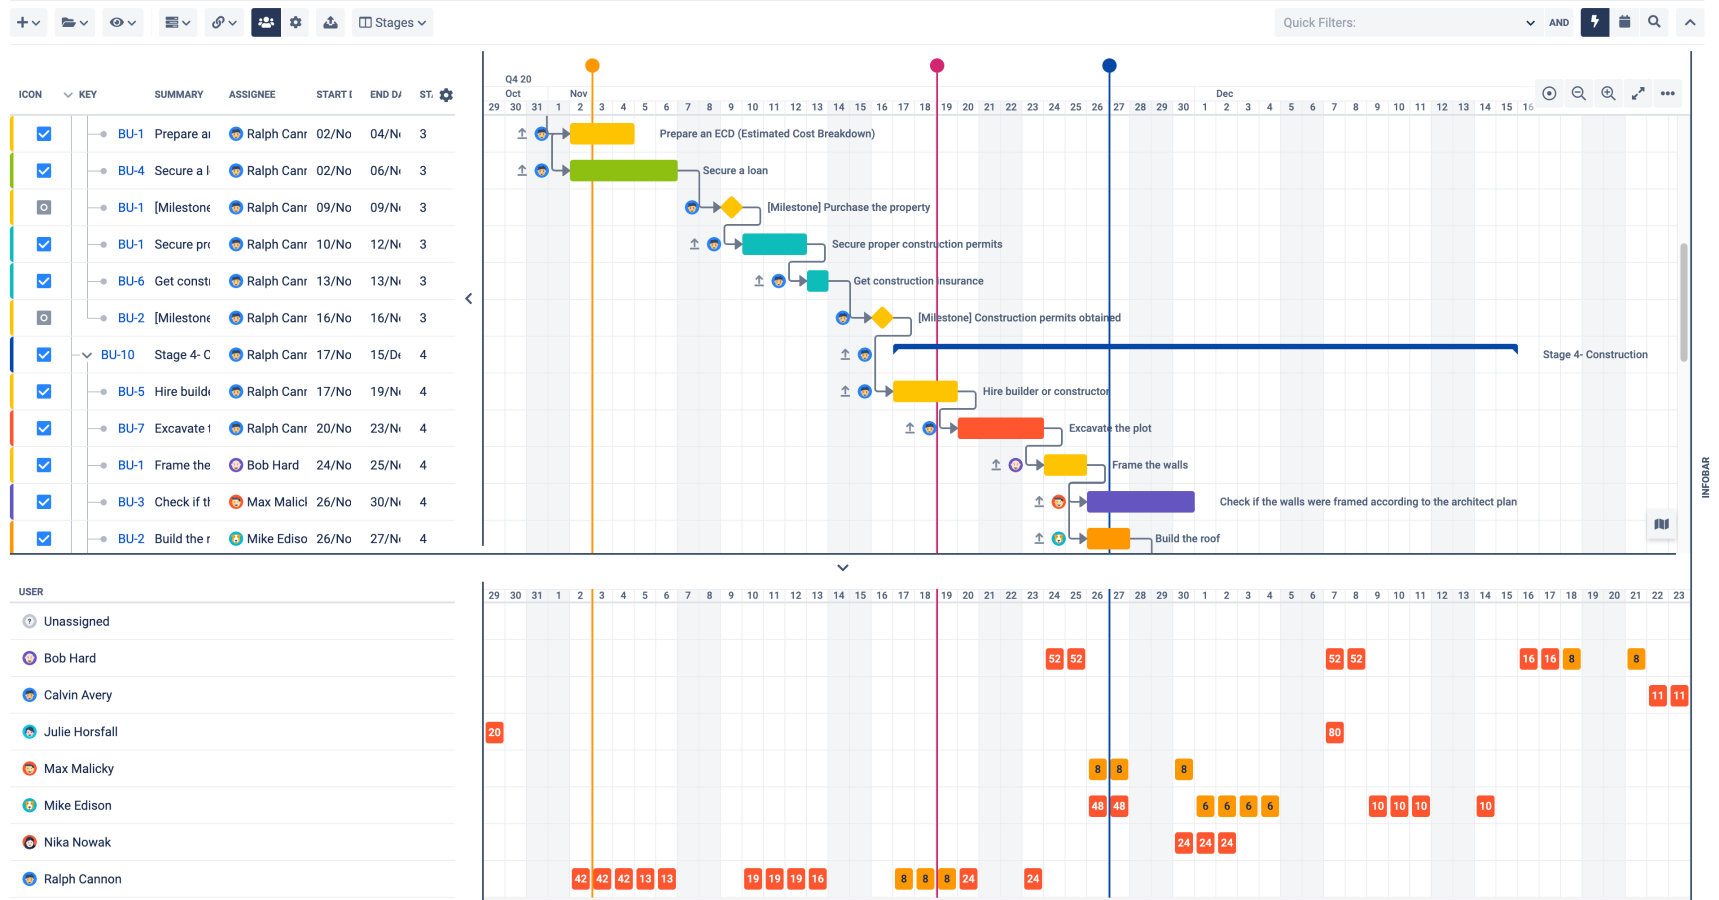
\includegraphics[width=0.90\textwidth]{Bilder/Gantt.png}
	\caption{Beispiel für ein Gantt-Chart}
	\label{fig:Gantt}
\end{figure}


%=======================================================================
\section{Gliederung}
%=======================================================================
Die Gliederung verknüpft die Aufgabenstellung mit der Lösung. Ein Beispiel könnte lauten: "`Kapitel \ref{sec:BasicRulez} beschreibt die theoretischen Grundlagen usw."'


%=======================================================================
% Titelseite
%=======================================================================
\chapter{Theoretische Grundlagen}
\label{sec:BasicRulez}

\begin{figure}[h]
	\centering
		
\includegraphics[width=0.80\textwidth]{Bilder/Python_God.jpg}
	\caption{Es gibt Regeln an die man sich halten sollte \cite{Python83}}
	\label{fig:Python_God}
\end{figure}
In diesem Unterkapitel "`Theoretische Grundlagen"' soll ein Überblick über die unterschiedlichen Definitionen und Ansätze zum jeweiligen Thema und eine Abgrenzung zu verwandten Themen und Begriffen erfolgen \cite[S.~27]{Karm2011}.
Wissenschaftliche Arbeiten sollen Klarheit beim Leser hervorrufen.
Das bedeutet, dass der Leser die beschriebenen Sachverhalte exakt in der beabsichtigten Weise ohne Rückfragen verstehen muss.
Welche Definitionen sind relevant um den Bericht ohne weitere Hintergrundkenntnisse in dem Themenbereich zu verstehen?
Inhalte müssen logisch gegliedert und klar nachvollziehbar sein.
Es ist ein hohes Maß an Systematik, Ordnung, Logik und Klarheit erforderlich \cite[S.~1~ff.]{Hering2009}.

"`Zwischendurch müssen Sie immer wieder einmal die gedankliche Position des Lesers einnehmen und sich fragen:
\begin{itemize}
	\item Wann braucht der Leser welche Information?
	\item Fällt das hier verwendete Bild 'vom Himmel'?
	\item Soll ich mich auf die Gliederung beziehen, eine Zwischenzusammenfassung machen oder den neuen Dokumentteil aus übergeordneter Sicht ankündigen?
	\item Ist die Aufteilung der Informationen logisch und nachvollziehbar?"' \cite[S.~29]{Hering2009}.
\end{itemize}

Die nachfolgenden Grundregeln sind strikt zu beachten. 

% Zur besseren Übersicht können Abschnitte in Dateien ausgelagert werden.
\section{Grundlegender Aufbau}
Auf eine Überschrift folgt immer ein Absatz mit Text, \textbf{nie unmittelbar} eine Überschrift niedrigeren Ranges \cite[S.~197]{Balz2008}.\footnote{Hervorhebungen werden durch Kursivschrift oder halbfette Schrift realisiert. Vermieden werden soll Hervorhebung durch Unterstreichen, größere Schrift oder Großbuchstaben \cite[S.~182]{Balz2008}. Ebenfalls ungünstig ist die farbliche Hervorhebung von Wörtern oder Überschriften.}
Daher muss von der Einleitung eine schlüssige Überleitung zum Hauptteil und den anstehenden Unterkapiteln erfolgen.
Falls mehrere Versuche innerhalb des Praktikums durchgeführt werden, sollte an dieser Stelle kurz darauf eingegangen werden.

Ein Hauptkapitel (Kapitel mit nur einer Zählnummer) beginnt jeweils auf einer neuen Seite.
Innerhalb der Gliederung ist zu beachten, dass Gliederungsebene vier nicht überschritten werden sollte.
Die Unterteilung soll möglichst in der dritten Stufe enden \cite[S. 12]{Hering2009}.

Zum Beispiel soll eine Gliederungsebene "`2.2.1.3"' vermieden werden, also wird die Untergliederung bei Ebene "`2.2.1"' beendet.
Desweiteren muss darauf geachtet werden, dass ein Oberpunkt der Gliederung mindestens zwei Unterpunkte besitzt muss \cite[S. 53]{Karm2011}.
Dennoch sollen die Zählnummern innerhalb einer Hierarchiestufe nicht größer als neun werden \cite[S.~12]{Hering2009}.
Die jeweils übergeordneten Kapitel sollen einen Überblick über die Inhalte geben, die in den Unterkapiteln thematisiert sind.
In den Überblicken sollte jedoch kein zusätzliches Wissen vermittelt werden \cite[S.~196]{Balz2008}.

In diesem Dokument wird ein beispielhaftes Inhaltsverzeichnis für einen Praktikumsbericht aufgezeigt, der u.a. im Praktikum Grundlagen der Elektrotechnik an der HSHL angefertigt werden muss.
Die Inhaltsübersicht und das Inhaltsverzeichnis sollen einen Überblick über die Systematik der Arbeit geben und einen "`ersten Eindruck"' vermitteln.
Man sollte sich bewusst sein, dass das Inhaltsverzeichnis die erste Information ist, die ein Leser von der Arbeit aufnimmt \cite[S.~49]{Karm2011}.
Die Gliederung soll bereits als "`roter Faden"' dienen.
Für den Leser ist die Gliederung der wichtigste Schlüssel zum Erfassen des Inhalts.
Wissenschaftliche Arbeiten erfordern ein hohes Maß an Ordnung und Logik, welche sich auch in der Gliederung widerspiegeln muss \cite[S.~9 ~ff.]{Hering2009}.

\noindent
Üblicherweise gliedert sich der inhaltliche Aufbau in Einleitung, Hauptteil und Schluss.
Die Einleitung beinhaltet die Aufgabenstellung und die Motivation der wissenschaftlichen Arbeit (s. Einleitung, S. \pageref{sec:Einleitung}).
Im Hauptteil werden die theoretischen Grundlagen erläutert und der Lösungswegs sowie die Ergebnisse dargestellt.
Die Ergebnisse werden im Schlussteil in Kurzform wiedergegeben und kritisch diskutiert.
Weitere Untergliederungen dieser drei Hauptpunkte können je nach Art der wissenschaftlichen Arbeit und den entsprechenden Anforderungen umgesetzt werden.
In dieser wissenschaftlichen Arbeit werden die benötigten Gliederungspunkte für einen Praktikumsbericht aufgezeigt.

Ein Praktikumsbericht, der die Beschreibung einen Versuchs beinhaltet, sollte unbedingt folgende Unterpunkte beinhalten:
\begin{enumerate}
\item Theoretische Grundlagen 
\item Aufgabenstellung mit Versuchsbeschreibung
\item Versuchsvorbereitung (benötigter Materialien und Beschreibung des Versuchsaufbaus)
\item Versuchsdurchführung
\item Versuchsauswertung (vgl. \cite{Hering2009}, S. 18)
\end{enumerate}

Als allgemeine Gliederung für ingenieurwissenschaftliche Arbeit (z.\,B Bachelor- oder Masterarbeit) empfiehlt sich die Nachfolgende. 

Titelseite\\
Inhaltsverzeichnis
\begin{enumerate}
	\item Einleitung (Einführung in die Aufgabenstellung)
  \item Theoretische Grundlagen
	\item Lösungsweg ggf. Lösungsalternative
  \item Ergebnis
  \item Zusammenfassung (mit anschl. Diskussion der Ergebnisse) und Ausblick
\end{enumerate}
Quellenverzeichnis\\
Anhang\\
Eidesstattliche Erklärung 

%---------------------------------------------
\section{Stilistische Anforderungen}
%---------------------------------------------
Die "`Ich"'- oder "`Wir"'-Perspektive soll im gesamten Textteil vermieden werden.
Stattdessen sollte aus der dritten, neutralen Person oder in Passivkonstruktionen geschrieben werden \cite[S.~130]{Hering2009}.
Die wissenschaftliche Arbeit darf nicht im Sinne eines Erlebnisberichtes sondern als sachorientierte Dokumentation aufgefasst werden. 
Eine Ausnahme besteht im Schlussteil, in dem der Autor eine kritische Auseinandersetzung mit der Thematik einbringen darf.

Ein wesentliches Kriterium für die Verständlichkeit der Inhalte ist ein wissenschaftlich-technischer, konkreter, klarer und präziser Sprachstil.
Es sollte auf keinen Umständen Umgangssprache verwendet werden. 
Folgende Punkte sorgen für bessere Textverständlichkeit:
\begin{itemize}
	\item Kurze Sätze bilden.
	\item Möglichst nur einen Hauptsatz mit einem oder zwei Nebensätzen bzw. zwei mit Semikolon verknüpfte Hauptsätze verwenden. 
	\item Nicht zu viele Nebensätze in Klammern sondern als alleinstehende Sätze oder in Fußnoten unterbringen.
	\item "`Welcher, welche, welches"' als Relativpronomen sind veraltet und sollen ersetzt werden durch "`der, die, das"'. 
	\item Ein- und überleitende Sätze verwenden, um Ihre Leser mit Worten zu führen.
Damit können Sie:\\
\begin{itemize}
	\item die Gliederung bzw. das Inhaltsverzeichnis aufgreifen,
	\item den bisher beschriebenen Sachverhalt zusammenfassen,
	\item zum nächsten Dokumentteil überleiten oder
	\item einen neuen Dokumentteil einleiten.
\end{itemize}
	\item Anschaulich formulieren, in Bildern sprechen!
	Analogien, Metaphern und Vergleiche erzeugen Assoziationen beim Leser.
	Dadurch kann der Leser Ähnlichkeiten und Abweichungen von dem ihm bereits bekannten Wissen leichter erkennen \cite[S.~129]{Hering2009}.
	\item Konjunktive vermeiden.
	\item Apostrophe sparsam im Text verwenden.
	\item Indirekte statt direkte Zitate verwenden.
	\item Wiederholungen von Wörtern in Sätzen vermeiden.
	\item Füllwörter, d.\,h. Wörter die beim Weglassen keinen Einfluss auf den Inhalt haben, vermeiden.
	\item Inhaltliche Blöcke im Text bilden und diese durch Einrückungen voneinander trennen.
\end{itemize}

\noindent
Die Erzählzeit ist das Präsens (Gegenwart).
Das Imperfekt (Vergangenheit) wird nur bei Beschreibung eines früher verwendetes Bauteil, Messverfahren usw., eingesetzt.
Es sollten keine emotionsbeladenen und umgangssprachlichen Formulierungen verwendet werden \cite[S.~131]{Hering2009}.
Zur verständliche Formulierung gehören einleitende Sätze am Anfang eines Dokumentteils.
Zusammenfassende und überleitende Sätze sollten am Ende eines Dokumentteils eingebracht werden.
Diese Sätze können auch Einsatz zur Ein- und Überleitung bei Bildern und Tabellen finden.
Sie beschreiben z.B. welche Informationen und warum als nächstes folgen, wie die folgenden Informationen zu bewerten sind, welchen Stellenwert die zuvor beschriebenen Informationen haben usw. (vgl. \cite{Hering2009}, S. 136 f.).

Technische Geräte sollen grundsätzlich nach ihrer Funktion benannt werden.
Zum Beispiel ist die Bezeichnung Antriebsrad besser als Zahnrad oder Halteplatte eindeutiger als Platte.
Technische Verfahren werden zur Veranschaulichung funktionsgerecht benannt.
So sollte die Bezeichnung "`Variante 1"' in z.\,B. "`elektrisch-mechanische Lösung"' umbenannt werden \cite[S.~131]{Hering2009}.
Dabei muss aber beachtet werden, dass keine Worte erfunden werden dürfen.
Es sollen nur Worte verwendet werden, die im Duden stehen.
Bezeichnungen wie z.B. "`bestromen"' oder "`anflanschen"' sollten in einer wissenschaftlichen Arbeit durch gebräuchliche Ausdrücke ersetzt werden.

Bei der Benutzung von Fachbegriffen, Fremdwörten und Abkürzungen gilt es eine angemessene Verwendung einzuhalten.
Fremdsprachige Wörter sollten vermieden werden.
Nach Möglichkeit sollen die sinngemäßen Bezeichnungen in der deutschen Sprache verwendet werden.
Ausnahme bilden fremdsprachige Fachausdrücke, bei denen eine Übersetzung ins Deutsche übertrieben erscheinen würde (sogenannte Anglizismen vermeiden).
Bei der Verwendung von Fachbegriffen müssen diese bei erstmaliger Verwendung erläutert werden.
Dies kann sowohl innerhalb des Textes als auch in Fußnoten erfolgen.\footnote{In den Fußnoten können Anmerkungen untergebracht werden ohne den Lesefluss zu stören.
In die Fußnoten gehören ausschließlich zusätzliche Informationen und Anmerkungen, die als nennenswert erachtet werden, aber nicht für die Argumentation erforderlich sind. Jede Fußnote beginnt mit einem Großbuchstaben und endet mit einem Punkt \cite[S.~197~f.]{Balz2008}.}
Unbekannte Abkürzungen werden ebenfalls beim ersten Auftreten definiert \cite[S.~136]{Balz2008}.
Sobald eine Abkürzung einmalig eingeführt wurde, muss sie konsequent verwendet werden.
Beim Einführen einer Abkürzung wird zuerst der vollständige Begriff genannt und in Klammern auf die Abkürzung verwiesen wird.
Bei mehr als fünf verwendeten Abkürzungen sollte ein Abkürzungsverzeichnis erstellt werden.


%===================================================================================================================
\subsection{Zitieren}
Sobald auf fremde Literaturquellen referenziert wird, ist die Verwendung einer korrekten Zitierweise und der Aufbau eines Literatur- und Quellenverzeichnis erforderlich.
Die Inhalte fremder Quellen können in einem direkten oder indirekten Zitat wiedergegeben werden.

Bei der wörtlichen Übernahme einer fremden Quelle im eigenen Text wird von einem direkten Zitat gesprochen.
Dieses steht immer in Anführungszeichen und muss buchstaben- und zeichengetreu übernommen werden, auch wenn das Original Rechtschreib- oder sonstige Fehler enthält.

Ein indirektes Zitat liegt vor, wenn fremde Gedanken und Ausführungen sinngemäß übernommen werden.
Es steht nie in Anführungszeichen und wird z.\,B. mit einem "`vgl."' referenziert.

Man spricht von einem Vollbeleg, wenn ein gesondertes Literaturverzeichnis vorliegt und auf die Einträge im Literaturverzeichnis verwiesen wird wie das in dieser wissenschaftlichen Arbeit der Fall ist.
Bei einem Kurzbeleg existiert kein gesondertes Literaturverzeichnis.
Die Quellen der Zitate werden dabei innerhalb des Textes oder in Fußnoten aufgeführt \cite{Kipp2012}.

Sinngemäß zitierte Sachverhalte werden durch die Quellenangabe z.\,B. am Ende eines Teilsatzes, eines Satzes oder Absatzes gekennzeichnet \cite[S.~109~ff.]{Hering2009}.
Eine wissenschaftliche Arbeit stützt sich nicht nur auf Schriftwerke, sondern auch auf andere geschützte Werke der Literatur, Wissenschaft und Kunst.
Der Textteil beinhaltet neben den eigenen und zitierten Inhalten auch Abbildungen, Tabellen und Gleichungen, welche an entsprechenden Stellen in den Text eingebunden werden \cite[S.~196]{Balz2008}.
Die Theorie ist mit entsprechenden Zitaten, Formeln, Tabellen und Bildern aus Fachliteratur zu belegen.
Dabei sollen grundsätzlich Primärquellen den Sekundärquellen vorgezogen werden.
Primärquellen oder Originalquellen sind eigenständige wissenschaftliche Arbeiten, die einen konkreten Betrachtungsgegenstand haben und zum Zeitpunkt der Veröffentlichung neue Erkenntnisse über diesen liefern \cite[S.~81]{Balz2008}.

"`Schwierige und komplexe Inhalte brauchen Wahrnehmungshilfen [...]: Dazu zählen Überschriften, Auszeichnungen, Bilder, Symbole und Strukturbilder, Tabellen und Diagramme, Fotos und multimediale Elemente"' (\cite{Balz2008}, S. 28).
Wenn Formeln und Gleichungen verwendet werden, so werden sie nicht in den Text eingebettet sondern nehmen eine eigene Zeile ein. 
Es ist üblich, die Gleichungen zusätzlich mit Gleichungsnummern am rechten Rand des Satzspiegels zu kennzeichnen, damit man sich im Text auf die jeweilige Gleichung beziehen kann.
Im gesamten Text kann auf die Formeln Bezug genommen werden indem ihre Nummer genannt wird.
Dabei werden die Klammern weggelassen \cite[S.~133~ff.]{Hering2009}.
Nachfolgend wird ein Beispiel für das korrekte Einbringen einer Formel mit dem dazugehörigen Querverweis im Text dargestellt.

Nach Gleichung \ref{eq:Gleichung1} errechnet sich die Gesamtsystemleistung $P_{ges}$ aus dem Produkt von Spannung $U_f$, Strom $I_f$ und der Anzahl der LEDs $n$.

\begin{equation}
P_{ges} = P_E = I_f \cdot U_f \cdot n
\label{eq:Gleichung1}
\end{equation}

\noindent
Formeln treten selten als einzelne Formel wie in Gleichung \ref{eq:Gleichung1} auf.
Meist erscheinen sie im Rahmen umfangreicherer Berechnungen mit mehreren Formeln und Umformungen.
Innerhalb des Textes sollten die Formelgrößen erklärt, Formelumformungen beschrieben und die Ergebnisse aufgegriffen werden.
Die Einflussgrößen, die in einer Formel auftreten, werden im Text kurz vor oder direkt nach der Formel benannt und erläutert \cite[S.~134]{Hering2009}.
Es folgt ein Beispiel für eine umfangreichere Berechnung.

Die LEDs sind mit einem Durchflussstrom von $700\,mA$ und einer Durchflussspannung von $3,31V$ klassifiziert.
Um die benötigte Systemleistung $P_{ges}$ aufzubringen, wird von dem typischen Durchflussstrom von $700\,mA$ ausgegangen.
Bei diesem stellt sich nach Gleichung \ref{eq:Spannung319V} eine Durchflussspannung von $3,19\,V$ ein und erreicht bei der Anzahl $n$ von 14 LEDs somit die Gesamtsystemleistung von $31,25\,W$.
%
\begin{align}
P_{ges} = P_E &= I_f \cdot U_f \cdot n \\
\Leftrightarrow U_f	&= \frac{P_{ges}}{I_f \cdot n}\\
	  &= \frac{31,25W}{700mA \cdot 14}\\
	  &= 3,19V
\label{eq:Spannung319V}
\end{align}

Gleichungen sowie Zahlen mit Einheiten werden kursiv hervorgehoben, falls diese im Textteil erscheinen.
Mit Latex gesetzte Formeln sehen einheitlich aus, da Formelzeichen in der mathematischen Umgebung grundsätzlich kursiv dargestellt werden.

%===================================================================================================================
\subsection{Quellen}
Fertigen Sie Ihr Literaturverzeichnis nach DIN ISO 690:2013-10 ist an.
Die DIN ISO 690:2013-10 sieht im Literaturverzeichnis zwingend die Nennung des Urhebers, Sachtitels, Auflage und Erscheinungsvermerke wie Erscheinungsort, Verlag und Erscheinungsjahr einer Literaturquelle vor.
\newpage
Dies sind Beispiele für Zitate nach DIN ISO 690:2013-10:

\textbf{Bücher}
  \begin{tabbing}
    [1]x \= Mitte  \kill
    $[1]$ \> \textsc{Paul, R.}: \textit{Elektrotechnik 1.} Berlin: Springer-Verlag, 3. Auflage 1993.\\
		\> ISBN: 978-0-387557-53-3\\
		$[2]$ \> \textsc{Balzert, H. u.a.}: \textit{Wissenschaftliches Arbeiten.} \\
		\> Witten: W3L-Verlag, 2. Auflage 2008. ISBN 987-3-937137-59-9\\
		$[3]$ \> \textsc{Eichler, H.-J.; Kronfeldt, H.-D.; Sahm, J.}: \textit{Das neue Physikalische Grund-}\\
		\>\textit{praktikum.} Berlin, Heidelberg: Springer-Verlag, 3. Auflage 2016.\\
		\> ISBN: 978-3-662490-22-8
  \end{tabbing}

\textbf{Internetquellen}
  \begin{tabbing}
    [1]x \= Mitte  \kill
    [4] \> \textsc{Wikipedia}: \textit{Feldlinien.} URL: \url{https://de.wikipedia.org/wiki/Feldlinien}, \\
		\>Abruf: 12.02.2022\\
  \end{tabbing}

\textbf{Zeitschriften}
  \begin{tabbing}
    [1]x \= Mitte  \kill
    [5] \> \textsc{Zhong, X.;Lewis, J. M.}: \textit{A New Method for Autonomous Robot Calibration.} \\
		\>In: Proc. of the IEEE Int. Conf. on Robotics and Automation. \\
		\>IEEE, 1995, S. 1790-1795 Vol.2. DOI: 10.1109/ROBOT.1995.525529.\\
  \end{tabbing}




%================================================================================================================================================
\subsection{Verwendung von Bildern}
Die verbale Darstellung von Informationen ist zwar exakt aber nicht sehr anschaulich.
Nach dem Prinzip "`ein Bild sagt mehr als tausend Worte"' können viele Sachverhalte einfacher und klarer in Form von Bildern dargestellt werden als es durch verbale Beschreibung möglich ist.
Die Inhalte sollten grafisch dargeboten werden, weil sie so leichter aufgenommen und verarbeitet werden können \cite[S.~67]{Hering2009}.
Es ist wichtig eine geeignete Darstellungsform für die Veranschaulichung der theoretischen Inhalte zu finden.
Dies müssen nicht unbedingt Abbildungen, sondern können auch Tabellen, Diagramme oder andere Darstellungsformen sein.

"`Grafiken, Tabellen und Fotos, die aus einer fremden Quelle übernommen wurden, müssen mit einem entsprechenden Verweis auf den Ursprung versehen werden.
Eigenerstellte Inhalte werden nicht explizit gekennzeichnet"' \cite[S.~111]{Balz2008}.
Wie in Abbildung \ref{fig:KompassSensor} zu sehen ist, setzt sich die Abbildungsunterschrift aus Nummerierung, gefolgt von der Benennung und der Quellenangabe zusammen. 
Bei der Abbildungsunterschrift sowie Tabellenüberschriften wird auf das Satzzeichen am Ende des Satzes verzichtet.
In der Regel gilt bei Abbildungen und Tabellen eine horizontal zentrierte Anordnung, da das optische Erscheinungsbild dadurch ausgewogen erscheint \cite[S.~183]{Balz2008}.
Für die Abbildungsunterschrift sowie Tabellenüberschrift gilt ebenfalls eine zentrierte Anordnung.

\begin{figure}[h]
	\centering
		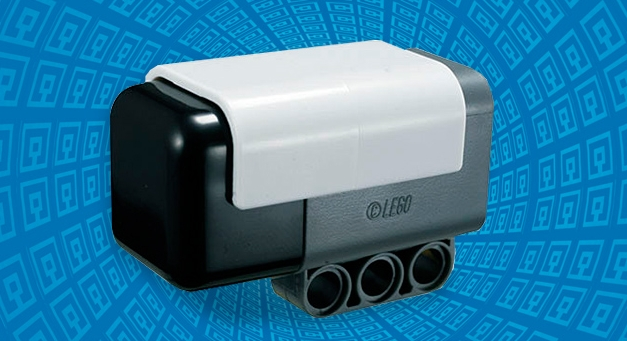
\includegraphics[width=0.5\textwidth]{KompassSensor.jpg}\\
			\caption{Kompasssensor für Lego Mindstorms NXT und EV3 \cite{Lego12}}
		\label{fig:KompassSensor}
\end{figure}

\noindent
Bilder und Tabellen werden entweder durch die ganze wissenschaftliche Ausarbeitung chronologisch durchnummeriert wie es in dieser wissenschaftlichen Arbeit gehandhabt wird.
Oder die Nummern werden aus der Kapitelnummer und einer laufenden Nummer innerhalb des Kapitels kombiniert \cite[S.~15]{Hering2009}.

Jede Abbildung muss als Querverweis im Text referenziert werden \textbf{bevor} diese im Dokument erscheint.
Auf jedes Bild muss im Text mindestens einmal hingewiesen werden.
Dabei soll eine Verbindung zwischen Bild und Text geschaffen werden und das Bild möglichst in der Nähe des Hinweises im Text erscheinen.
Falls von mehreren Stellen auf ein Bild hingewiesen wird, dann sollte das Bild in der Nähe des wichtigsten Hinweises angeordnet werden \cite[S.~76]{Hering2009}.

Bei der Auswahl der Abbildung muss darauf geachtet werden, dass diese in angemessener Druckqualität vorliegt.
Die Qualität kann durch ein Bildbearbeitungsprogramm optimiert werden, indem der Kontrast oder die Schärfe angepasst wird.
Grundsätzlich sollte eine Abbildung nur Informationen beinhalten, die im Text beschrieben werden.
Damit das Bild übersichtlich bleibt, sollte in Abbildungen nur das Wesentliche dargestellt werden.
Durch das Weglassen und Vereinfachen von Elementen in der Abbildung wird beim Leser die Konzentration auf das Wesentliche gelenkt \cite[S.~70~f.]{Hering2009}.

Der Übersichtlichkeit halber sollten auf einer Textseite nicht mehr als zwei Abbildungen, Tabellen oder andere Visualisierungsformen abgebildet werden.
Generell sollten Abbildungen nur dann eingesetzt werden, wenn es notwendig ist, komplexe Inhalte darzustellen, nicht als bloße Dekoration.
Wenn innerhalb der Abbildung schriftliche Anteile enthalten sind, sollte die Schriftgröße leserlich oder optimalerweise so groß wie die verwendete Schriftgröße im Text sein.
Es sollte vermieden werden, dass ein Bild unbekannte Fachbegriffe enthält oder dass in Text und Bild unterschiedliche Bezeichnungen für gleiche Gegenstände oder Sachverhalte auftreten \cite[S. 80]{Hering2009}.






%\include{Kapitel/Typografie}


\chapter{Darstellung der möglichen Lösungswege}
\label{cha:Loesungswege}

Sie haben bereits die Problemstellung beschrieben und die fachlichen Grundlagen geschaffen. In diesem Kapitel werden mögliche Lösungswege beschrieben. Häufig gibt es verschiedene Lösungswege, daher gehen Sie in den folgenden wissenschaftlichen Schritten vor. Sie
\begin{enumerate}
	\item beschreiben die mögliche Lösungswege anhand eines Morphologischen Kastens, 
	\item entwickeln Bewertungskriterien für die Lösung,
	\item bewerten die sinnvollen Lösungsalternativen und
	\item wählen anhand der Auswahlkriterien einen Lösungsweg aus und begründen Ihre Wahl sachlich.
\end{enumerate}

%===================================================================================================
\section{Materialien}
Die, für einen Versuch notwendigen, Materialien werden hier präzise mit Artikelbezeichung und Anzahl in Form einer Auflistung aufgeführt. 
Folgende Angaben müssen unbedingt gemacht werden:

\begin{itemize}
	\item Prüfmaschine / Versuchseinrichtung mit Hersteller, Typbezeichnung, Inventarnummer usw.
	\item alle jeweils an der Maschine bzw. Einrichtung eingestellten Parameter
	\item alle Messgeräte, jeweils mit Hersteller, Typbezeichnung, Inventarnummer, eingestellten Parametern usw.
	\item verwendete Proben mit allen erforderlichen Angaben nach der jeweiligen DIN-, EN-, ISO-Norm bzw. andere Normen je nach Notwendigkeit
	\item bei nicht genormten Versuchen sinngemäße Angaben zur Probenform, zu Versuchsparametern, zu Temperaturen, physikalischen und chemischen Eigenschaften usw.
	\item sämtliche gemessenen Werte bzw. Versuchsergebnisse mit allen Parametern
	\item angewendete Auswertungsformeln mit vollständigen Quellenangaben usw. \cite[S.~24]{Hering2009}.
\end{itemize}

%================================================================================================
\section{Versuchsaufbau...}
"`...wird in diesem Kapitel beschrieben."'
Dieses Beispiel soll zeigen, dass der Dokumentteil-Titel sprachlich nicht in den darauffolgenden Text einbezogen werden darf.
Der erste Satz des nachfolgenden Textes muss deshalb ein vollständiger Satz sein, der jedoch die Sachaussage des Dokumentteil-Titels aufgreifen bzw. wiederholen darf.
Hinter der Dokumentteil-Nummer und dem Dokumentteil-Titel darf nie ein Satzzeichen wie Punkt, Doppelpunkt, Fragezeichen, Ausrufungszeichen usw. stehen \cite[S.~14~f.]{Hering2009}.

\chapter{Darstellung der Ergebnisse}
In diesem Kapitel setzen Sie den zuvor ausgewählten Lösungsweg systematisch um. Sie beschreiben die Umsetzung und dokumentieren die Ergebnisse zu denen Sie gekommen sind. Es ist denkbar, dass das Ergebnis lautet: "`Dieser Lösungsweg schien laut Kapitel \ref{cha:Loesungswege} vielversprechend, hat jedoch das Problem nicht gelöst."' Diese Erkenntnisse sind jedoch auch wichtig und richtig und sollten im nachfolgenden Kapitel diskutiert werden.

\section{Versuchsdurchführung}
In diesem Abschnitt beschreiten Sie Ihren Lösungsweg. Dokumentieren Sie alles, was nötig ist, um Ihre Ergebnisse zu reproduzieren.

\section{Versuchsauswertung}
Die Versuchsauswertung erfolgt anhand der gemessenen Daten in Form von Messwerttabellen, Diagrammen und Abbildungen.
Tabellen besitzen immer eine Kopfzeile und eine Führungsspalte.
Die Kopfzeile enthält die Oberbegriffe zu den Spalten und die Führungsspalte Oberbegriffe zu den Zeilen.
Die Begriffe in der Kopfzeile und in der Führungsspalte sollen in sich konsistent und logisch gleichwertig sein \cite[S.~51]{Hering2009}.
Innerhalb der wissenschaftlichen Arbeit sollte eine gleich bleibende Tabellengestaltung beibehalten werden.
Die Eintragungen in den Zellen einer Tabelle können Zahlen, Wörter, Skizzen oder Kombinationen aus diesen Elementen sein.
Für die Eintragungen gelten die normalen Regeln der Groß- und Kleinschreibung, d.\,h. vor allem Adjektive beginnen mit kleinen Buchstaben.
Texte werden innerhalb der Zellen linksbündig ausgerichtet, da eine zentrierte Textausrichtung ein oft zu unruhiges Layout ergibt.
Die Tabellennummern können durch den ganzen Bericht hindurch fortlaufend hochgezählt werden wie es in dieser Ausarbeitung gehandhabt wurde.
Sie können jedoch auch zusammengesetzt werden aus der Kapitelnummer und der innerhalb eines Kapitels fortlaufend hoch gezählten Tabellennummer \cite[S.~54~ff.]{Hering2009}.

In der nachfolgenden Tabelle \ref{tbl:Laplace} wird veranschaulicht wie Tabellen in den Bereicht eingebunden werden\footnote{Auf jede im Text angeordnete Tabelle sollte im Text mindestens einmal hingewiesen werden (vgl. \cite{Hering2009}, S. 58).}.
In diesem Beispiel werden die Tabellennummern durch den Bericht hindurch fortlaufend hochgezählt.
Die Tabellen\textbf{überschrift} mit Nummerierung und Benennung steht im Gegensatz zu Grafiken zentriert oberhalb der Tabelle.
Grafische Abbildungen wie Fotos oder Screenshots werden üblicherweise in unveränderter Form mit Quellenverweis übernommen.
Tabellen sollten jedoch neu erstellt werden, wobei die Inhalte aus der fremden Quelle übernommen werden, damit durchgängig die gleiche Schriftart und -größe verwendet wird \cite[S.~113]{Balz2008}.

\begin{table*}[h]
	\centering
	\caption{Laplace Transformation, Quelle: \cite{Kiencke2001}}
	\label{tbl:Laplace}
		\begin{tabular}[t]{|l|l|l|}
		\hline
		allg. Eigenschaft / Operation & Zeitfunktion $f(t)$ & Bildfunktion $F(s)$\\ \hline
		Linearität & $a_{1}f_{1}(t)+a_{2}f_{2}(t)$ & $a_{1}F_{1}(s)+a_{2}Ff_{2}(s)$\\ \hline
		Ähnlichkeitssatz & $f(at)$ & $\frac{1}{a}F(\frac{s}{a})$ für $a>0$\\ \hline
		Verschiebung im Originalbereich & $f(t-a)$ & $e^{-as}F(s)$\\ \hline
		Verschiebung im Bildbereich & $e^{-at}\cdot{f(t)}$ & $F(s+a)$ mit $(a\in{C})$\\ \hline
		Sinus-Multiplikation & $sin(at)\cdot{f(t)}$ & $\frac{1}{2i}(F(s-ia)-F(s+ia))$\\ \hline
		Cosinus-Multiplikation & $cos(at)\cdot{f(t)}$ & $\frac{1}{2}(F(s-ia)+F(s+ia))$\\ \hline
		\end{tabular}
\end{table*}

\noindent
Bei kleineren Tabellen wird bewirkt, dass Informationen sehr systematisch, übersichtlich und strukturiert dargestellt werden.
Im Gegensatz dazu wirken größere Tabellen oft unübersichtlich.
Es fällt dem Leser einer großen Zahlen-Tabelle meist schwer, Verhältnisse von Zahlen abzuschätzen und Größen miteinander zu vergeleichen.
Deshalb sollte man große Zahlen-Tabellen in Diagrammform visualisieren.
Trotzdem müssen die Berechnungen, statistischen Auswertungen und Versuchsergebnisse mit exakten Zahlen belegt werden.
Die umfangreichen Zahlen-Tabellen können im Anhang untergebracht werden.
Im Text erscheinen aussagekräftige Visualisierungen und die zugehörigen Tabellen werden mit einem Verweis auf den Anhang referenziert \cite[S.~52]{Hering2009}.

Bei Diagrammen gilt als Grundprinzip, dass eindeutige Beschriftungen von Achsen, Säulen, Sektoren usw. erforderlich sind.
Graphen mit farbigen Kurven sollten immer eine Legende besitzen.
Oft kann die Verständlichkeit eines Diagramms auch dadurch gesteigert werden, dass die Aussage als Titel bzw. Beschriftung direkt über oder neben dem Diagramm erscheint. 
Ein Beispiel, wie Diagramm und Titel bzw. Beschriftung zusammenwirken können, zeigt Abbildung 2 \cite[S.~84~f.]{Hering2009}.

\begin{figure}[h]
	\centering
		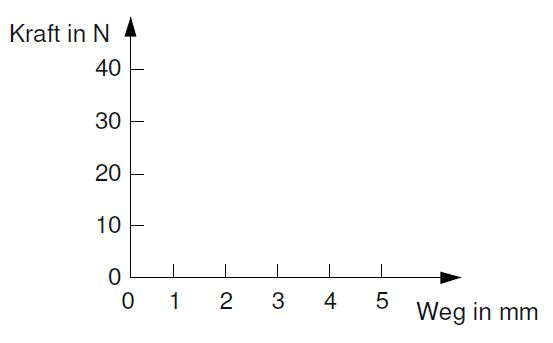
\includegraphics[width=0.6\textwidth]{Diagramm1.jpg}\\
			\caption{Beispielhaftes Diagramm zur Verdeutlichung der Anordnung nach \cite{Hering2009}}
		\label{fig:Diagramm1}
\end{figure}

\noindent
Alle Diagramme und Bilder erhalten eine Bildunterschrift mit Bildnummer.
Dabei sollte die Anordnung und Formatierung der Bildunterschriften einheitlich sein.
Die Achsen müssen genau beschriftet werden mit Achsenbezeichnung (als Text oder Formelbuchstabe) und zugehöriger Maßeinheit, Maßzahlen und Pfeilen an den Achsenenden (die Pfeile zeigen nach oben und rechts).
Eine horizontale Text-Angabe sowie die waagerechte Beschriftung der Achsen ist unbedingt vorzuziehen, weil die Grafik so nicht gedreht werden muss.
Wenn ein Diagramm zum Ablesen von Zahlen dient, dann ist die Verwendung von Netzlinien vorteilhaft.
Solbald in einem Diagramm mehrere Kurven eingezeichnet werden sollen, müssen die Kurven eindeutig zu unterscheiden sein.
Dafür können verschiedene Farben, Linienarten und Messpunktsymbole verwendet werden \cite[S.~85~ff.]{Hering2009}.
\chapter{Zusammenfassung und Ausblick}
Der Schlussteil besteht aus einer kurzen Zusammenfassung und kann auch persönliche Bemerkungen, Bewertungen etc. enthalten. Zuerst wird somit das Vorher geschriebene knapp zusammengefasst. Anschließend werde die Ergebnisse reflektiert. Die Zusammenfassung setzt sich kritisch mit der Aufgabenstellung auseinander und beantwortet die Fragen:
\begin{itemize}
	\item Was sollte getan werden und was wurde tatsächlich erreicht?
	\item Wo gab es besondere Schwierigkeiten?
	\item Welche Teile der Aufgabenstellung konnten eventuell gar nicht bearbeitet werden und warum?
\end{itemize}

Der Ausblick kann Empfehlungen für eine weitere sinnvolle Fortsetzung des Projektes bzw. der Forschungsarbeit enthalten.
Solche Empfehlungen beruhen üblicherweise auf Erkenntnissen, die während der Bearbeitung des laufenden Projektes entstanden sind \cite[S.~44]{Hering2009}.

Es wird darauf hingewiesen, dass die wissenschaftliche Arbeit am Ende unbedingt von einer dritten Person korrekturgelesen werden sollte.
Dadurch können Fehlerarten wie falsche Wortwahl, Rechtschreibfehler. Zeichensetzungsfehler, Grammatikfehler, Stilfehler, inhaltliche Wiederholungen, Fehler im logischen Gedankenfluss, Layout-Fehler sowie sonstige Fehler aufgedeckt werden \cite[S.~174]{Hering2009}.
Zudem wird der Autor beim häufigen Lesen der eigenen Texte mit der Zeit "`betriebsblind"' gegenüber den eigenen Formulierungen.
Auch aus diesem Grund sollte von einem Außenstehenden überprüft werden, ob der Bericht für Projektfremde verständlich ist \cite[S.~130]{Hering2009}.

% ANH?NGE
\begin{appendix}
%=======================================================================
% Anhang A
%=======================================================================

%---------------------------------------
\chapter{Versuchs- und Messprotokolle}
\label{cha:AnhangA}
%---------------------------------------

Im Anhang werden ergänzende Dokumente untergebracht, die im Textteil wegen ihres Umfangs keinen Platz gefunden haben.
Der Anhang darf auf keinen Fall größer als der Umfang des Textteils sein und wird nicht zum Seitenumfang des Textteils hinzugerechnet \cite[S.~198~f.]{Balz2008}.
Falls die beigelegten Dokumente nicht gebunden werden sollen, können sie in eine separate Mappe eingelegt oder auf einem Datenträger abgegeben werden.
In diesem Fall sollte ein Vermerk wie "`in separatem Ordner"' oder "`als CD-Rom angefügt"' im Anhang hinzugefügt werden. Sprechen Sie dies mit der Betreuenden Person ab. Vielleicht ist ein Link auf einen SVN-Tag ausreichend und Sie können sich die Arbeit erleichtern.


%XXXXXXXXXXXXXXXXXXXXXXXX-----Kapitel-----XXXXXXXXXXXXXXXXXXXXXXXXXXX
%XXXXXXXXXXXXXXXXXXXXXXXXXXXXXXXXXXXXXXXXXXXXXXXXXXXXXXXXXXXXXXXXXXXX
%XXXXXXXXXXXXXXXXXXXXXXXXXXXXXXXXXXXXXXXXXXXXXXXXXXXXXXXXXXXXXXXXXXXX
%Kapitel Vorlage für Bilder, Formeln, etc......
\chapter{Vorlagen für LaTeX}
\label{Kapitel_Vorlage}
%XXXXXXXXXXXXXXXXXXXXXXXXXXXXXXXXXXXXXXXXXXXXXXXXXXXXXXXXXXXXXXXXXXXX
%XXXXXXXXXXXXXXXXXXXXXXXXXXXXXXXXXXXXXXXXXXXXXXXXXXXXXXXXXXXXXXXXXXXX
%XXXXXXXXXXXXXXXXXXXXXXXXXXXXXXXXXXXXXXXXXXXXXXXXXXXXXXXXXXXXXXXXXXXX


%XXXXXXXXXXXXXXXXXXXXXXXX-----Sektion-----XXXXXXXXXXXXXXXXXXXXXXXXXXX
%XXXXXXXXXXXXXXXXXXXXXXXXXXXXXXXXXXXXXXXXXXXXXXXXXXXXXXXXXXXXXXXXXXXX
\section{Sektion Vorlage}
\label{Sektion_Vorlage}
%XXXXXXXXXXXXXXXXXXXXXXXXXXXXXXXXXXXXXXXXXXXXXXXXXXXXXXXXXXXXXXXXXXXX
%XXXXXXXXXXXXXXXXXXXXXXXXXXXXXXXXXXXXXXXXXXXXXXXXXXXXXXXXXXXXXXXXXXXX

%XXXXXXXXXXXXXXXXXXXXXXXX-----Subsektion--XXXXXXXXXXXXXXXXXXXXXXXXXXX
\subsection{Subsektion Vorlage}
\label{Subsektion_Vorlagen}
%XXXXXXXXXXXXXXXXXXXXXXXXXXXXXXXXXXXXXXXXXXXXXXXXXXXXXXXXXXXXXXXXXXXX


%XXXXXXXXXXXXXXXXXXXXXXXX-----MiniSek--------XXXXXXXXXXXXXXXXXXXXXXXX
\minisec{MiniSek} \label{MiniSek_Vorlagen}
%XXXXXXXXXXXXXXXXXXXXXXXXXXXXXXXXXXXXXXXXXXXXXXXXXXXXXXXXXXXXXXXXXXXX

%XXXXXXXXXXXXXXXXXXXXXXXX-----Paragraf-------XXXXXXXXXXXXXXXXXXXXXXXX
\paragraph{Paragraf Vorlage} \label{Paragraf_}
%XXXXXXXXXXXXXXXXXXXXXXXXXXXXXXXXXXXXXXXXXXXXXXXXXXXXXXXXXXXXXXXXXXXX


%-----------------------------Gleichung------------------------------
\begin{equation}
 \label{Gleichung_1}
\end{equation}
%--------------------------------------------------------------------


%-----------------------------mehrere Gleichungen--------------------
\begin{eqnarray}
\label{Gleichung_2}
 \nonumber
 &=&
 \\
 &=&
 \\
\end{eqnarray}
%--------------------------------------------------------------------


%-----------------------------Aufzählung-----------------------------
\begin{Aufzaehlung}{$\bullet$}
\item
blabla
\item
blabla
\end{Aufzaehlung}
%--------------------------------------------------------------------



%Ein Bild kann man so "`einbinden"': (Der Ausdruck "`clip="'
%verhindert, dass das Bild über seine
%Boundingbox überläuft, das hei{\ss}t es ist auf keinen Fall grö{\ss}er!)
%


%///////////////////////////// Bild /////////////////////////////////
\begin{figure}[h!]\begin{center}
 
\includegraphics[width=\BildBreiteGross, clip=]{Calvin_und_Hobbes2}
 %[width=15cm,height=8cm,scale=0.5,angle=45]
 \caption{Calvin und Hobbes \cite{Watterson2013}}
 %\label{Bild_}
\end{center}\end{figure}
%////////////////////////////////////////////////////////////////////

%///////////////////////////// 2 Bilder nebeneinander ///////////////
\begin{figure}[h!]\centering
 \subfloat[Bildbeschreibung subfigure 1]
    {\label{Bild_subfigure_1}
    
\includegraphics[width=\BildSubfigureBreite]{Calvin_und_Hobbes2}}
 \subfloat[Bildbeschreibung subfigure 2]
    {\label{Bild_subfigure_2}
    
\includegraphics[width=\BildSubfigureBreite]{Calvin_und_Hobbes2}}
 \caption{Hauptbildunterschrift}
\end{figure}
%////////////////////////////////////////////////////////////////////

\begin{figure}[h!]\centering
\captionsetup[subfloat]{labelformat=empty} % (a), (b) unterdrücken
 \subfloat[]
    {\label{fig:Bild_subfigure_1}
    
\includegraphics[width=0.45\textwidth]{Calvin_und_Hobbes2}}
    \hspace{0.5 cm}
 \subfloat[]
    {\label{fig:Bild_subfigure_2}
    
\includegraphics[width=0.45\textwidth]{Calvin_und_Hobbes2}}
 \caption{Zählpfeile und Vorzeichen des Stromes}
 \captionsetup[subfloat]{labelformat=parens}
\end{figure}

% Beschrifttung unterdrückt

%-----------------------------Tabelle--------------------------------
\begin{table}[h!]
  \centering
  \renewcommand{\arraystretch}{1.5}
  \begin{tabular}{|p{5.3cm}|p{10cm}|} \hline
    t&t
    \\\hline\hline
    t&t
    \\\hline
    \end{tabular}
  \caption{Versuchstabelle}
  \label{Tabelle_Versuch}
\end{table}
%--------------------------------------------------------------------




%-----------------------------Aufzählung-----------------------------
\begin{list}{\bullet}{
 \setlength{\leftmargin}{4cm}
 \setlength{\labelsep}{1cm}
 \setlength{\labelwidth}{4cm}}

\item[Punkt 1] bla bla bla ldfkjasdhfjlk hjkadhfas jk
dkashfjkas hjkdf hajks ajd jkf

\item[Punkt 2]

\item[Punkt 3]

\end{list}
%--------------------------------------------------------------------





Rotierter Text (erst in ps oder pdf sichtbar):

\begin{rotate}{90}
Rotiert?
\end{rotate}

\vspace{2cm}

\begin{rotate}{90}
$H + 4 -\frac{3}{4}$
\end{rotate}




$_K\vec{r}_{C2} = [l_{C2} \quad 0 \quad 0 ]^T$

 $_I\vec{e}_1$

Gänsefüsschen   "`Text"'

Einheiten:

$[\frac{kgm^2}{s}]$ für die Dämpfung

$[\frac{rad}{s}]$ für Winkelgeschwindigkeiten

$[\frac{kgm^2rad}{s^2}]$ für die Reibung



$_I\vec{e}_1$

$\dot{q}_2x$


Link auf eine Homepage
\href{http://de.wikipedia.org/wiki/Welt}{hier}



Matrizen kann man als "`Tabellen"' aufschreiben:
%--------------------------------------------------------------------
 %\begin{displaymath} {^{KI}\mf{A}=}
%\label{Matrix_A_K_I_Beispiel} \left(
%\begin{array}{ccc}

%\cos{q_2}\cos{\beta}+\sin{q_2}\sin{\alpha}\sin{\beta}
%&\sin{q_2}\cos{\alpha}
%&-\cos{q_2}\sin{\beta}+\sin{q_2}\sin{\alpha}\cos{\beta}\\

%-\sin{q_2}\cos{\beta} + \cos{q_2}\sin{\alpha}\sin{\beta}
%&\cos{q_2}\cos{\alpha}
%&\sin{q_2}\sin{\beta}+\cos{q_2}\sin{\alpha}\cos{\beta}\\

%\cos{\alpha}\cos{\beta} &-\sin{\alpha}
%&\cos{\alpha}\cos{\beta}

%\end{array}
%\right)
%\end{displaymath}\\
%--------------------------------------------------------------------



Matrizen kann man besser so aufschreiben:
%--------------------------------------------------------------------
%\begin{equation}
%^{KI}\mf{A}=
%\begin{pmatrix}
%
%\cos{\beta}        &0       &-\sin{\beta}\\
%
%0                  &1       &0\\
%
%\sin{\beta}        &0       &\cos{\beta}
%
%\end{pmatrix}
%\end{equation}
%--------------------------------------------------------------------


Für Vektoren
%--------------------------------------------------------------------
\begin{equation}\label{Matrix_A_K_alpha_Beispiel}
\boxed{ _K\vec{r}_{C2}=
\begin{pmatrix}
ls2\\0\\0
\end{pmatrix}}
\end{equation}
%--------------------------------------------------------------------


Aufzählung selbst gestalten:
\begin{list}{$\bullet$}{\setlength
        {\leftmargin}{0.5cm}}
        \item Zusatzlenkwinkel durch das AFS-System
        \item Stellung eines Zusatzmoments
\end{list}




%XXXXXXXXXXXXXXXXXXXXXXXXXXXXXXXXXXXXXXXXXXXXXXXXXXXXXXXXXXXXXXXXXXXX
%XXXXXXXXXXXXXXXXXXXXXXXXXXXXXXXXXXXXXXXXXXXXXXXXXXXXXXXXXXXXXXXXXXXX
\section{Sektion Versuche}
\label{Sektion_Versuche}
%XXXXXXXXXXXXXXXXXXXXXXXXXXXXXXXXXXXXXXXXXXXXXXXXXXXXXXXXXXXXXXXXXXXX
%XXXXXXXXXXXXXXXXXXXXXXXXXXXXXXXXXXXXXXXXXXXXXXXXXXXXXXXXXXXXXXXXXXXX
Test für Formelzeichen: Im Text funktioniert diese mbox gut:
\mbox{$x = y$}.
%-----------------------------Gleichung------------------------------
\begin{equation}
 Sogar in Formeln kann man die mbox mit integrierter Formel
 verwenden:
 x = y, \mbox{$x = y$}
\end{equation}
%--------------------------------------------------------------------


Partialbruchzerlegung:
%--------------------------------------------------------------------
\begin{eqnarray*}
 f(t) = \frac{As + B}{s^3(J s^2 + d s + c)} &=&
 -{\frac {cJB+dcA-{d}^{2}B}{{c}^{3}s}}
 \\
 &&
 +{\frac {cA-dB}{{c}^{2}{s}^{2}}}
 +{\frac {B}{c{s}^{3}}}
 \\
 &&
 +{\frac
 {-{d}^{3}B-J{c}^{2}A+2\,cJdB+{d}^{2}cA+s{J}^{2}cB+sJdcA
 -sJ{d}^{2}B}{{c}^{3}\left
 (J{s}^{2}+ds+c\right )}}
\end{eqnarray*}
%--------------------------------------------------------------------

%XXXXXXXXXXXXXXXXXXXXXXXX-----Kapitel-----XXXXXXXXXXXXXXXXXXXXXXXXXXX
%XXXXXXXXXXXXXXXXXXXXXXXXXXXXXXXXXXXXXXXXXXXXXXXXXXXXXXXXXXXXXXXXXXXX
%XXXXXXXXXXXXXXXXXXXXXXXXXXXXXXXXXXXXXXXXXXXXXXXXXXXXXXXXXXXXXXXXXXXX
\chapter{Tipps und Tricks}
%XXXXXXXXXXXXXXXXXXXXXXXXXXXXXXXXXXXXXXXXXXXXXXXXXXXXXXXXXXXXXXXXXXXX
%XXXXXXXXXXXXXXXXXXXXXXXXXXXXXXXXXXXXXXXXXXXXXXXXXXXXXXXXXXXXXXXXXXXX
%XXXXXXXXXXXXXXXXXXXXXXXXXXXXXXXXXXXXXXXXXXXXXXXXXXXXXXXXXXXXXXXXXXXX

%XXXXXXXXXXXXXXXXXXXXXXXX-----Sektion-----XXXXXXXXXXXXXXXXXXXXXXXXXXX
%XXXXXXXXXXXXXXXXXXXXXXXXXXXXXXXXXXXXXXXXXXXXXXXXXXXXXXXXXXXXXXXXXXXX
\section{Vorgeschrieben Software}
%XXXXXXXXXXXXXXXXXXXXXXXXXXXXXXXXXXXXXXXXXXXXXXXXXXXXXXXXXXXXXXXXXXXX
%XXXXXXXXXXXXXXXXXXXXXXXXXXXXXXXXXXXXXXXXXXXXXXXXXXXXXXXXXXXXXXXXXXXX
Um Ihre Projektdaten nachhaltig weiterverwenden zu können, verwenden Sie bitte die Standardtools, die an der HSHL verfügbar sind:
\begin{itemize}
	\item Schaltungssimulation: NI Multisim
	\item Leiterplattenlayout: NI Ultiboard
	\item Modellbasierte Entwicklung: MATLAB/Simulink
	\item CAD: Solid Works
	\item Statische Codeanalyse: Polyspace
	\item Programmablaufpläne: \href{https://www.heise.de/download/product/papdesigner-51889}{PAP-Designer}
	\item Projektplanung: \href{https://www.heise.de/download/product/ganttproject-25167}{Gantt Project}
\end{itemize}



\section{Implementierung eines Internet-Links}
\verb|\href{http://de.wikibooks.org/wiki/LaTeX-Kompendium}{Lehrbuch}|

\end{appendix}


% Literaturverzeichnis anlegen
% =============================
%\bibliographystyle{plain}
%\bibliographystyle{Literatur/acm}      %engl. Lit.-Verz.

% sieht gut aus: Namen als Abk?rzung + Jahreszahl
\ifalphaDIN
    \bibliographystyle{Literatur/alphadin} % oder abbrv, alpha, plainnat
\else
    \bibliographystyle{gerplain}
\fi

%f?r natbib-Paket & dt. DIN-Zitate (funktioniert noch nicht)
%\citet erzeugt: G?bel (2007)
%\citep erzeugt: (G?bel 2007)
% Achtung: vorher noch \usepackage[sort&compress]{natbib} laden.
%\bibliographystyle{Literatur/natdin}

% alle B?cher, die im Text nicht zitiert werden, aber trotzdem im
% Literaturverzeichnis auftauchen sollen:
% \nocite{*}

%Literaturverzeichnis aus Datei laden, die mit wbibdb.exe oder jabref
%erstellt wurde
%f?r den Verzeichnisbaum in WinEdt (folgende Zeile auskommentiert lassen!)
%include "Literatur/MG_Literaturverzeichnis.bib"
\bibliography{Literatur/Literaturverzeichnis}

 






%=======================================================================
% Eidesstattliche Erklärung
%=======================================================================
\thispagestyle{empty}
{\textbf{\large Eidesstattliche Erklärung}}


Ich versichere hiermit, dass ich die vorliegende Arbeit selbstständig und nur unter Benutzung der angegebenen Literatur und Hilfsmittel angefertigt habe.
Wörtlich übernommene Sätze und Satzteile sind als Zitate belegt, andere Anlehnungen hinsichtlich Aussage und Umfang unter Quellenangabe kenntlich gemacht.
Die Arbeit hat in gleicher oder ähnlicher Form noch keiner Prüfungsbehörde vorgelegen und ist auch noch nicht veröffentlicht.

%An das Ende jeder Bachelorarbeit ist die Eidesstaatliche Versicherung auf eine gesonderte Seite zu setzen -> HSHL-Vorgabe!!
\vspace*{2 cm}

\begin{figure}[htbp]
		
\includegraphics[width=0.30\textwidth]{Bilder/Unterschrift.png}
	\label{fig:Unterschrift}
\end{figure}
\vspace*{-0.9cm}
Erika Müller % handschriftliche Unterschrift hierhin!!

\OrtDatum  

%%%%%%%%%%%%%%%%%%%%%%%%%%%%%%%%%%%%%%%%%%%%%%%%%%%%%%%%%%%%%%%%%%%%%
%%%
%%% Dokument fertig
%%%
%%%%%%%%%%%%%%%%%%%%%%%%%%%%%%%%%%%%%%%%%%%%%%%%%%%%%%%%%%%%%%%%%%%%%
\end{document}

